\chapter{Zero-intervals}
\label{intervals}
In Chapter~\ref{chap:chars}, we characterized matrices avoiding small patterns. Their structure is very dependent on the pattern and the results are hard to generalize for arbitrary patterns. In this chapter, we look for a more general property that restricts the complexity that a class of matrices can have.

\begin{defn}
For a matrix~$M\in\Mat$, a row interval $M[\{r\},[c_1,c_2]]$ is a \emph{zero-interval} if all entries are zero-entries, $c_1=0$ or $M[r,c_1-1]=1$ and $c_2=n$ or $M[r,c_2+1]=1$. In other words, it is an interval of zero-entries bounded by one-entries. Symmetrically, we also call a single column sequence $M[[r_1,r_2,\{c\}]]$ a \emph{zero-interval} if all entries are zero-entries, $r_1=0$ or $M[r_1-1,c]=1$ and $r_2=m$ or $M[r_2+1,c]=1$. In the same spirit, we define a \emph{one-interval} to be an interval of one-entries in a single line of $M$ bounded by zero-entries (or edges of the matrix).
\end{defn}

In the previous chapter, for pattern~$P\in\Pat$ it very often holds that any inclusion maximal matrix $M$ avoiding $P$ as an interval minor has at most $l$ zero-intervals in each row and at most $k$ zero-intervals in each column. The main goal of this chapter is to describe patterns for which the size of a pattern bounds the number of zero-intervals of any inclusion maximal matrix that avoids it.

$$P_1=\smm{ &\bullet& \\\bullet& & \\ & &\bullet}\ P_2=\smm{ &\bullet& \\ & &\bullet\\\bullet& & }\ P_3=\smm{\bullet& & \\ & &\bullet\\ &\bullet& }\ P_4=\smm{ & &\bullet\\\bullet& & \\ &\bullet& }$$

Ultimately, we show that for every matrix $P$, there is an inclusion maximal matrix $M\in\Avm{P}$ with arbitrarily many zero-intervals if and only if $P$ contains an interval minor $P_1,P_2,P_3$ or $P_4$.

\section{Pattern complexity}

Let us present some useful notion. First of all, every time we speak about a \emph{maximal} matrix of a class, we mean inclusion maximal -- it has no zero-entry that can be changed to a one-entry so that it still belongs to the class. In terms of pattern avoidance, maximal matrices are those for which a change of a zero-entry creates a mapping of the pattern (or possibly many mappings).

\begin{defn}
For any matrix $P$, let $\Avmax{P}$ be a set of all maximal matrices avoiding $P$ as an interval minor.
\end{defn}

\begin{defn}
Let $P$ be a pattern, let $e$ a one-entry of $P$, $M\in\Avm{P}$ and let $z$ be an arbitrary zero-interval of $M$. We say that $z$ is \emph{usable for} $e$ if there is a zero-entry contained in $z$ such that if we change it to a one-entry, it creates a mapping that uses the new one-entry to map $e$. This way, $z$ can be usable for many one-entries of $P$ at the same time. 
\end{defn}

\begin{obs}
Let $P\in\Pat$ and $M\in\Mat$ be matrices such that $\PnimM$. Let $z=M[\{r_1\},[c_1,c_2]]$ be a zero-interval of $M$ usable for a one-entry~$e=P[r,c]$. If we change a zero-entry of $z$ and create a mapping of $P$ that uses the changed entry to map $e$, then no such mapping can map column~$c$ outside of columns $[c_1,c_2]$ of $M$. 
\end{obs}
\begin{proof}
Since the changed entry is used to map $e$, clearly every mapping needs to use a column from $[c_1,c_2]$ to map column~$c$. If, for contradiction, after a change of a zero-entry there is a mapping using columns outside $[c_1,c_2]$ then it, without loss of generality. uses $c_1-1$ but since it bounds zero-interval~$z$, it is a one-entry and this one-entry can be used in the mapping instead of the changed entry, which gives us a contradiction with $\PnimM$.
\end{proof}

\begin{defn}
For a class of matrices $\class{M}$, we define its \emph{row-complexity}, $\rc{\class{M}}$ to be the supremum of the number of zero-intervals in a single row of any maximal $M\in\class{M}$. We say that $\class{M}$ is \emph{row-bounded}, if its row-complexity is finite, and \emph{row-unbounded} otherwise. Symmetrically, we define \emph{column-complexity}~$\cc{\class{M}}$ and the property of being \emph{column-bounded} and \emph{column-unbounded}. Class $\class{M}$ is \emph{bounded} if it is both row-bounded and column-bounded and it is \emph{unbounded} otherwise.
\end{defn}

\begin{defn}
We say that a set of pattern $\class{P}$ is \emph{bounding}, if the class $\Avm{\class{P}}$ is bounded and is \emph{non-bounding} otherwise.
\end{defn}

\begin{defn}
Let $\class{P}$ be a set of patterns and let $e$ be a one-entry of any $P\in\class{P}$. We define the \emph{row-complexity} of $e$, $\rce{\Avm{\class{P}}}{e}$ to be the supremum of the number of zero-intervals of a single row of any $M\in\Avmax{\class{P}}$ that are usable for $e$. We say that $e$ is \emph{row-unbounded} in $\Avm{\class{P}}$ if $\rce{\Avm{\class{P}}}{e}=\infty$ and \emph{row-bounded} otherwise. Symmetrically, we define the \emph{column-complexity}~$e$, $\cce{\Avm{\class{P}}}{e}$ to be the maximum number of zero-intervals of a single column of any matrix from $\Avmax{\class{P}}$ that are usable for $e$ and say $e$ is \emph{column-unbounded} if it is infinite and \emph{column-bounded} otherwise.
\end{defn}

The following observation follows directly from the definition and we use it heavily throughout the chapter to break symmetries.

\begin{obs}
\label{obs:transposebounded}
For every set $\class{M}$, $\class{M}$ is row-bounded if and only if $\class{M}^\top$ is column-bounded.
\end{obs}

\subsection{Adding empty lines}

Similarly, as we did in Chapter~\ref{chap:chars}, we show that we do not need to consider patterns with leading (and ending) empty rows (and columns).

\begin{obs}
For a matrix~$P\in\Pat$ and integer $n$, let $P'=P\hsum0^{k\times n}$. Matrix $P$ is bounding if and only if $P'$ is bounding. Moreover, if $P$ is bounding, then $\rc{\Avm{P'}}=\rc{\Avm{P}}+1$.
\end{obs}

\begin{lemma}
\label{lemma:twocols2}
Let $P\in\bin^{2\times k}$ and for any $l\geq1$ let $P^l\in\bin^{(l+2)\times k}$ be a pattern created from $P$ by adding $l$ new empty rows in between the two row of $P$. For every one-entry~$e$ of $P^l$ $\rce{\Avm{P^l}}{e}\leq k^2$.
\end{lemma}
\begin{proof}
Given $M\in\Avmax{P}$, let us look at an arbitrary row~$r$ of $M$. Without loss of generality assume $e=P[1,c]$. For contradiction, assume there are $k^2+1$ zero-intervals $z_1,\dots,z_{k^2+1}$ in $r$ usable for $e$.
\begin{itemize}
	\item $P[2,c]=1$: Clearly, there is a one-entry in rows $[r+l+1,m]$ underneath each $z_j$ and if we combine each such one-entry with a one-entry bounding corresponding $z_j$, we find a mapping of $\left(\{1\}^{2\times k^2}\right)^l$, contradicting $\PnimM$.
	\item $P[2,c]=0$: For each $i\in[t]$, we define an extended interval $z^*_i$ to be the interval containing $z_i$ and also all elements of $r$ between $z_i$ and $z_{i+1}$. Because of the Pigeonhole principle, we can find either $k$ consecutive extended intervals such that there are no one-entries in rows $[r+l+1,m]$ underneath them, or $k$ extended intervals such that there is a one-entry in rows $[r+l+1,m]$ underneath each of them. Because each extended interval contains a one-entry, in the second case we find $\left(\{1\}^{k\times2}\right)^l$ as an intervals minor. In the first case, without loss of generality, assume $P[2,c_1]=1$ and it is the minimum such $c_1>c$. Also let $z_{first},\dots,z_{last}$ be the consecutive zero-intervals. Now consider the mapping of $P^l$ created when a zero-entry of $z_{first}$ gets changed to a one-entry used to map $e$. Since $P[2,c_1]=1$ and there are no one-entries in rows $[r+l+1,m]$ underneath extended intervals $z_{first}$-$z_{last}$, $P^l[l+2,c_1]$ has to be mapped to the columns of $M$ after the end of $z_{last}$. This leaves $k$ one-entries to be used to map potential one-entries in $P^l[\{l+2\},[c,c_2-1]]$ and so $P^l\im M$.
\end{itemize}
\end{proof}

\begin{cor}
\label{cor:twocols}
Let $P\in\bin^{k\times2}$ and for any $l\geq1$ let $P^l\in\bin^{k\times(l+2)}$ be a pattern created from $P$ by adding $l$ new empty columns in between the two columns of $P$. Then $\Avm{P^l}$ is bounded for any $l\geq1$.
\end{cor}
\begin{proof}
We know $\Avm{P^l}$ is row-bounded from Lemma~\ref{lemma:twocols}. From Lemma~\ref{lemma:twocols2} and Observation~\ref{obs:transposebounded} we have that the class is also column-bounded.
\end{proof}

\subsection{Non-bounding patterns}
We see that for patterns having only two rows or columns we can indeed bound the number of zero-intervals of maximal matrices avoiding them. On the other hand, already for a pattern of size $3\times3$ we show that there are maximal matrices with arbitrarily many zero-intervals.

\begin{lemma}
\label{lemma:manyints}
Class $\Avm{P_1}$ is unbounded.
\end{lemma}
\begin{proof} For given $n$, let $M$ be a $(2n+1)\times(2n+1)$ matrix described by the picture:
$$\smm{	\bullet& &\bullet& &\bullet&\cdots&\bullet& &\bullet& &\bullet\\
		 & & & & &\cdots& & &\bullet&\bullet&\bullet\\
		 & & & & &\cdots& & &\bullet&\bullet&\bullet\\
		 & & & & &\cdots&\bullet&\bullet&\bullet& & \\
		 & & & & &\cdots&\bullet&\bullet&\bullet& & \\
		\vdots&\vdots&\vdots&\vdots&\vdots&\vdots&\vdots&\vdots&\vdots&\vdots&\vdots\\
		 & &\bullet&\bullet&\bullet&\cdots& & & & & \\
		 & &\bullet&\bullet&\bullet&\cdots& & & & & \\
		\bullet&\bullet&\bullet& & &\cdots& & & & & \\
		\bullet&\bullet&\bullet& & &\cdots& & & & & \\
		 }$$
We see that $P_1\nim M$ because we always need to map $P_1[2,1]$ and $P_1[3,3]$ to just one ``block'' of one-entries, which only leaves a zero-entry for $P_1[1,2]$.

If we change any zero-entry of the first row into a one-entry we get a matrix containing an interval minor of $\{1\}^{3\times3}$; therefore, containing $P_1$ as an interval minor. In case $M$ is not maximal, we can add some more one-entries to make it maximal but it will still contain a row with $n$ zero-intervals.
\end{proof}

Not only $M\in\Avmax{P_1}$ but it also avoids any $P\in\bin^{3\times3}$ such that $P_1\im P$. Its rotations avoid rotations of $P_1$ and we can deduce that a big portion of patterns of size $3\times3$ are non-bounding. Moreover, the result can be generalized also for bigger matrices.

\begin{thm}
For every $P$ such that $P_1\im P$, $\Avm{P}$ is unbounded.
\end{thm}
\begin{proof}
First, assume there is a mapping of $P_1$ into $P\in\Pat$ that assigns a one-entry of the first row to $P_1[1,2]$, a one-entry of the first column to $P_1[2,1]$ and a one-entry of the last row and column to $P_1[3,3]$. Then, we use a similar construction to what we did in the proof of Lemma~\ref{lemma:manyints} to find a matrix $M\in\Avmax{P}$ with $n$ zero-intervals for any $n$.

Let $P$ be an arbitrary pattern containing $P_1$ as an interval minor. Let $P[r_1,c_1],P[r_2,c_2]$ and $P[r_3,c_3]$ be one-entries that can be used to map $P_1[1,2],P_1[2,1]$ and $P_1[3,3]$ respectively. We take a submatrix~$P':=P[[r_1,r_3],[c_2,c_3]]$. Such a pattern fulfills assumptions of the more restricted case above and we can find a matrix $M'\in\Avmax{P'}$ having $n$ zero-intervals. We construct $M$ from $M'$ by simply adding new rows and columns containing only one-entries. We add $r_1-1$ rows in front of the first row and $k-r_3$ rows behind the last row. We also add $c_2-1$ columns in front of the first column and $l-c_3$ columns behind the last column. Constructed matrix~$M$ avoids $P$ an an interval minor because its submatrix $P'$ cannot be mapped to $M'$. At the same time, any change of a zero-entry of the $r_1$-th row of $M$ to a one-entry creates a copy of ${1}^{k\times l}$. Constructed $M$ can be seen in Figure~\ref{fig:manyints}.

\begin{figure}[!ht]
\centering
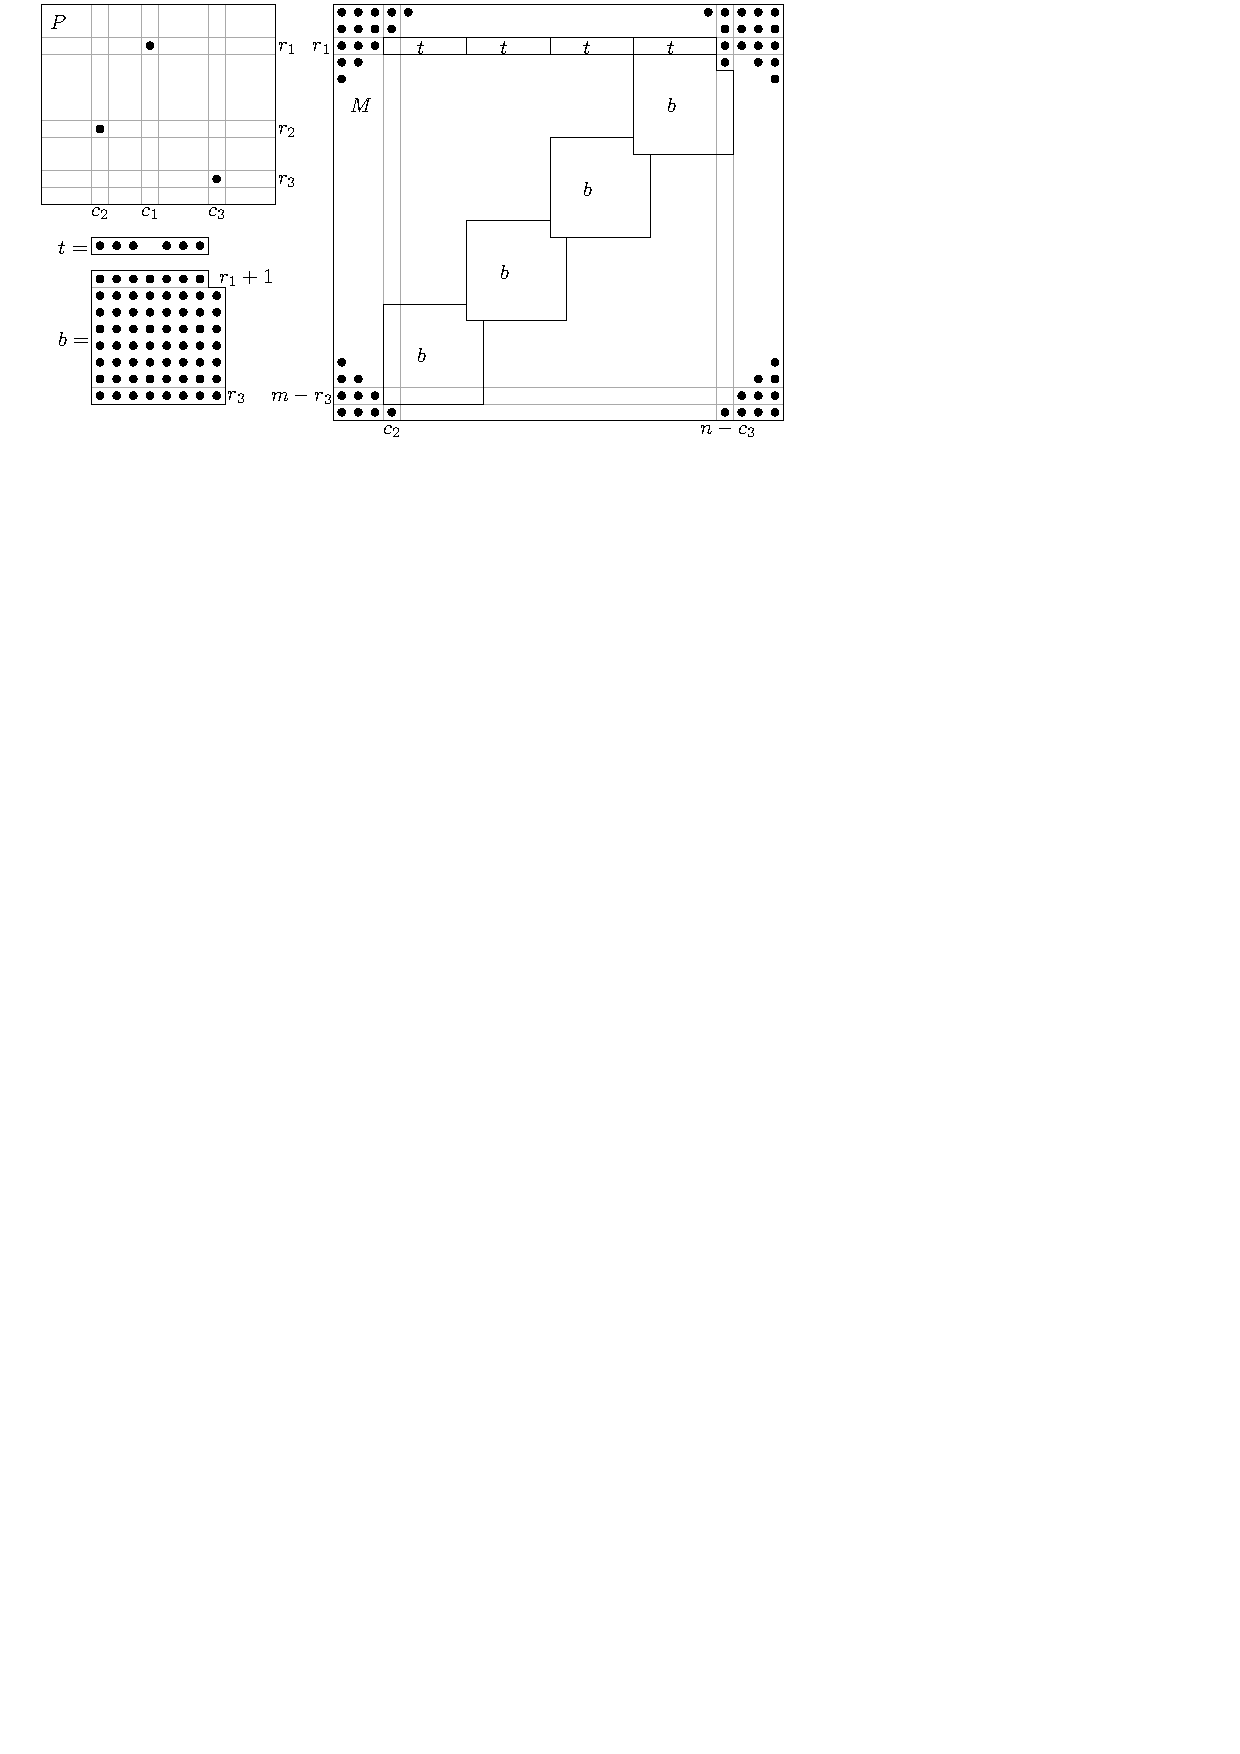
\includegraphics[width=120mm]{img/manyints.pdf}
\caption{Structure of a maximal matrix avoiding $P$ that has arbitrarily many one-intervals.}
\label{fig:manyints}
\end{figure}
\end{proof}

\subsection{Bounding patterns}

What makes it even more interesting is that any pattern avoiding all rotations of $P_1$ is already bounding.

\begin{thm}
\label{thm:boundedints}
Let $P$ be a pattern avoiding all rotations of $P_1$, then $P$:
\begin{enumerate}
	\item contains at most three non-empty lines or
	\item avoids $\smm{\bullet& \\ &\bullet}$ or $\smm{ &\bullet\\\bullet& }$.
\end{enumerate}
\end{thm}
\begin{proof}
Assume $P$ has four one-entries that do not share any row or column. Then those one-entries induce a $4\times4$ permutation inside $P$ and because $P$ does not contain any rotation of $P_1$, the induced permutation is either $1234$ or $4321$. Without loss of generality, assume it is the first one and denote its one-entries by $e_1,e_2,e_3$ and $e_4$.

For contradiction, assume $P$ also contains $P'=\smm{\bullet& \\ &\bullet}$. Clearly, no one-entry from $e_1,e_2,e_3$ and $e_4$ can be part of any mapping of $P'$ because it would induce a mapping of a rotation of $P_1$.

Let $e_2=P[r_2,c_2]$ and $e_3=P[r_3,c_3]$. The submatrix~$P[[r_2],[c_2,l]]$ avoids $P'$; otherwise, together with $e_1$ it would give us a rotated copy of $P_1$. Symmetrically, $P[[r_3,k],[c_3]]$ does not contain $P'$. Also, $P[[r_3-1],[c_3-1]]$ and $P[[r_2+1,k],[c_2+1,l]]$ are empty; otherwise, they would together with $e_2$ and $e_3$ give us a rotation of $P_1$. Up to rotation, the only possible way to have $P'\im P$ is that $P'[1,1]$ is mapped to a one-entry from $P[[r_3-1],[c_2,c_3-1]]$ but then this entry together with $e_1$ and $e_3$ give us a rotation of $P_1$, which is a contradiction.
\end{proof}

%%%%%%%%%%%%%%%%%%%%%%%%%%%%%%%%%%%%%%%%%%%%%%%%%% one non-empty line
\begin{lemma}
Let $P\in\Pat$ be a pattern having one non-empty line. Then $\rc{\Avm{P}}\leq k$ and $\cc{\Avm{P}}\leq l$.
\end{lemma}
\begin{proof}
Without loss of generality, let the non-empty line be a row~$r$. Consider any $M\Avmax{P}$. Matrices $M[[r-1],[n]]$ and $M[[m-r+1,m],[n]]$ contain no zero-entry. If we look at any other row, it cannot contain $k$ one-entries, so the maximum number of zero-intervals is $k$.

Consider a column~$c$ of $M$. If there is at least one one-entry in $M[[r,m-r],c]$ then because $M$ is maximal, the whole column is made of one-entries. Otherwise, there are two one-intervals $M[[r-1],c]$ and $M[[m-r,m],c]$.
\end{proof}

%%%%%%%%%%%%%%%%%%%%%%%%%%%%%%%%%%%%%%%%%%%%%%%%%% two non-empty lines
\begin{lemma}
Let $P\in\Pat$ be a pattern having two non-empty lines. Then $\rc{\Avm{P}}\leq k^2+l$ and $\cc{\Avm{P}}\leq l^2+k$.
\end{lemma}
\begin{proof}
First, we assume the two non-empty lines of $P$ are rows $r_1<r_2$ (or symmetrically columns). From Observation~\ref{obs:emptyrows} and maximality of $M$ we have that $M[[r_1-1],[n]]$ and $M[[m-r_2+1,m],[n]]$ contain no zero-entry. Therefore, we may restrict ourselves to the case when $r_1=1$ and $r_2=k$. From Corollary~\ref{cor:twocols}, we have that there are at most $k^2$ zero-intervals in each $M\in\Avmax{P}$.

Let the two non-empty lines of $P$ be a row~$r$ and a column~$c$. Because of symmetry, we only show the bound for rows. Let us take an arbitrary row of $M$ an look at its zero-intervals. For every one-entry~$e$ of the pattern except those in the $r$-th row, there is at most one zero-interval usable for $e$. For contradiction, assume there are two such zero-intervals $z_1$ and $z_2$. Let Figure~\ref{fig:twolines} illustrate the situation where dashed and dotted lines form mappings of an interval minor $P$ to $M$ when a zero-entry of $z_1$ and $z_2$ respectively is changed to a one-entry. When we take the outer two vertical and horizontal lines, we get a mapping of $P$ that can use an existing one-entry in between $z_1$ and $z_2$ to map $e$. This gives us a contradiction with $\PnimM$.

\begin{figure}[!ht]
\centering
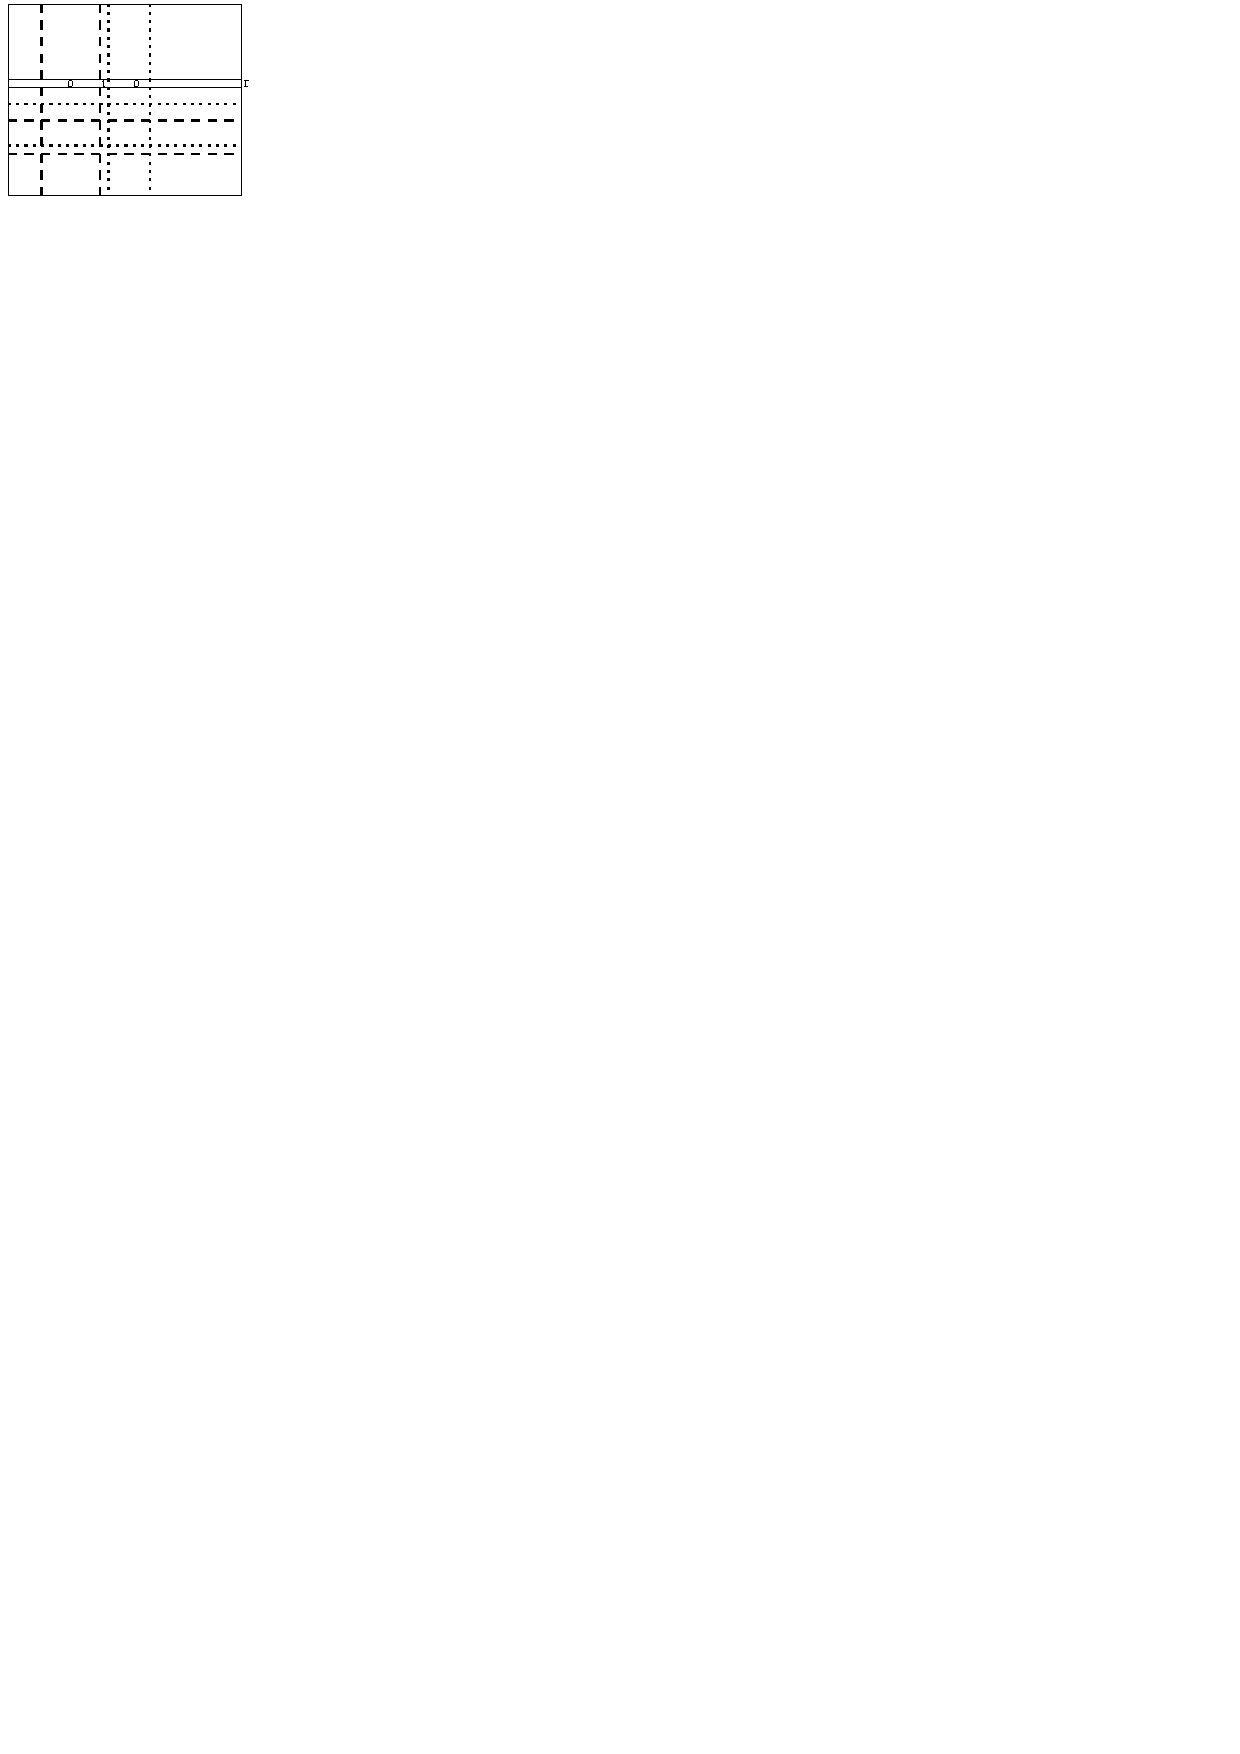
\includegraphics[width=70mm]{img/twolines.pdf}
\caption{Dashed and dotted lines resembling two different mappings of a forbidden pattern, where two horizontal lines show the boundaries of the mapping of row~$r$ and the vertical lines show boundaries of the mapping of column~$c$.}
\label{fig:twolines}
\end{figure}

For a one-entry $e=P[r,c']$, if $c'\leq c$ then there must be less than $c'$ one-entries before any zero-intervals usable for $e$; otherwise, we could map $P[r,[1,c']]$ just to the single row of $M$. It follows that $e$ is row-bounded. Symmetrically, the same holds in case $c'>c$ and together we have at most $k+l$ zero-intervals in each $M\in\Avmax{P}$.
\end{proof}

%%%%%%%%%%%%%%%%%%%%%%%%%%%%%%%%%%%%%%%%%%%%%% Lemma H
\begin{lemma}
\label{lemma:H}
Let $P\in\Pat$ be a pattern structured like one of the matrices in Figure~\ref{fig:lemmaH}. Then every one-entry in $P[\{r_2\},[c_1,c_2]]$ is row-bounded.

\begin{figure}[!ht]
\centering
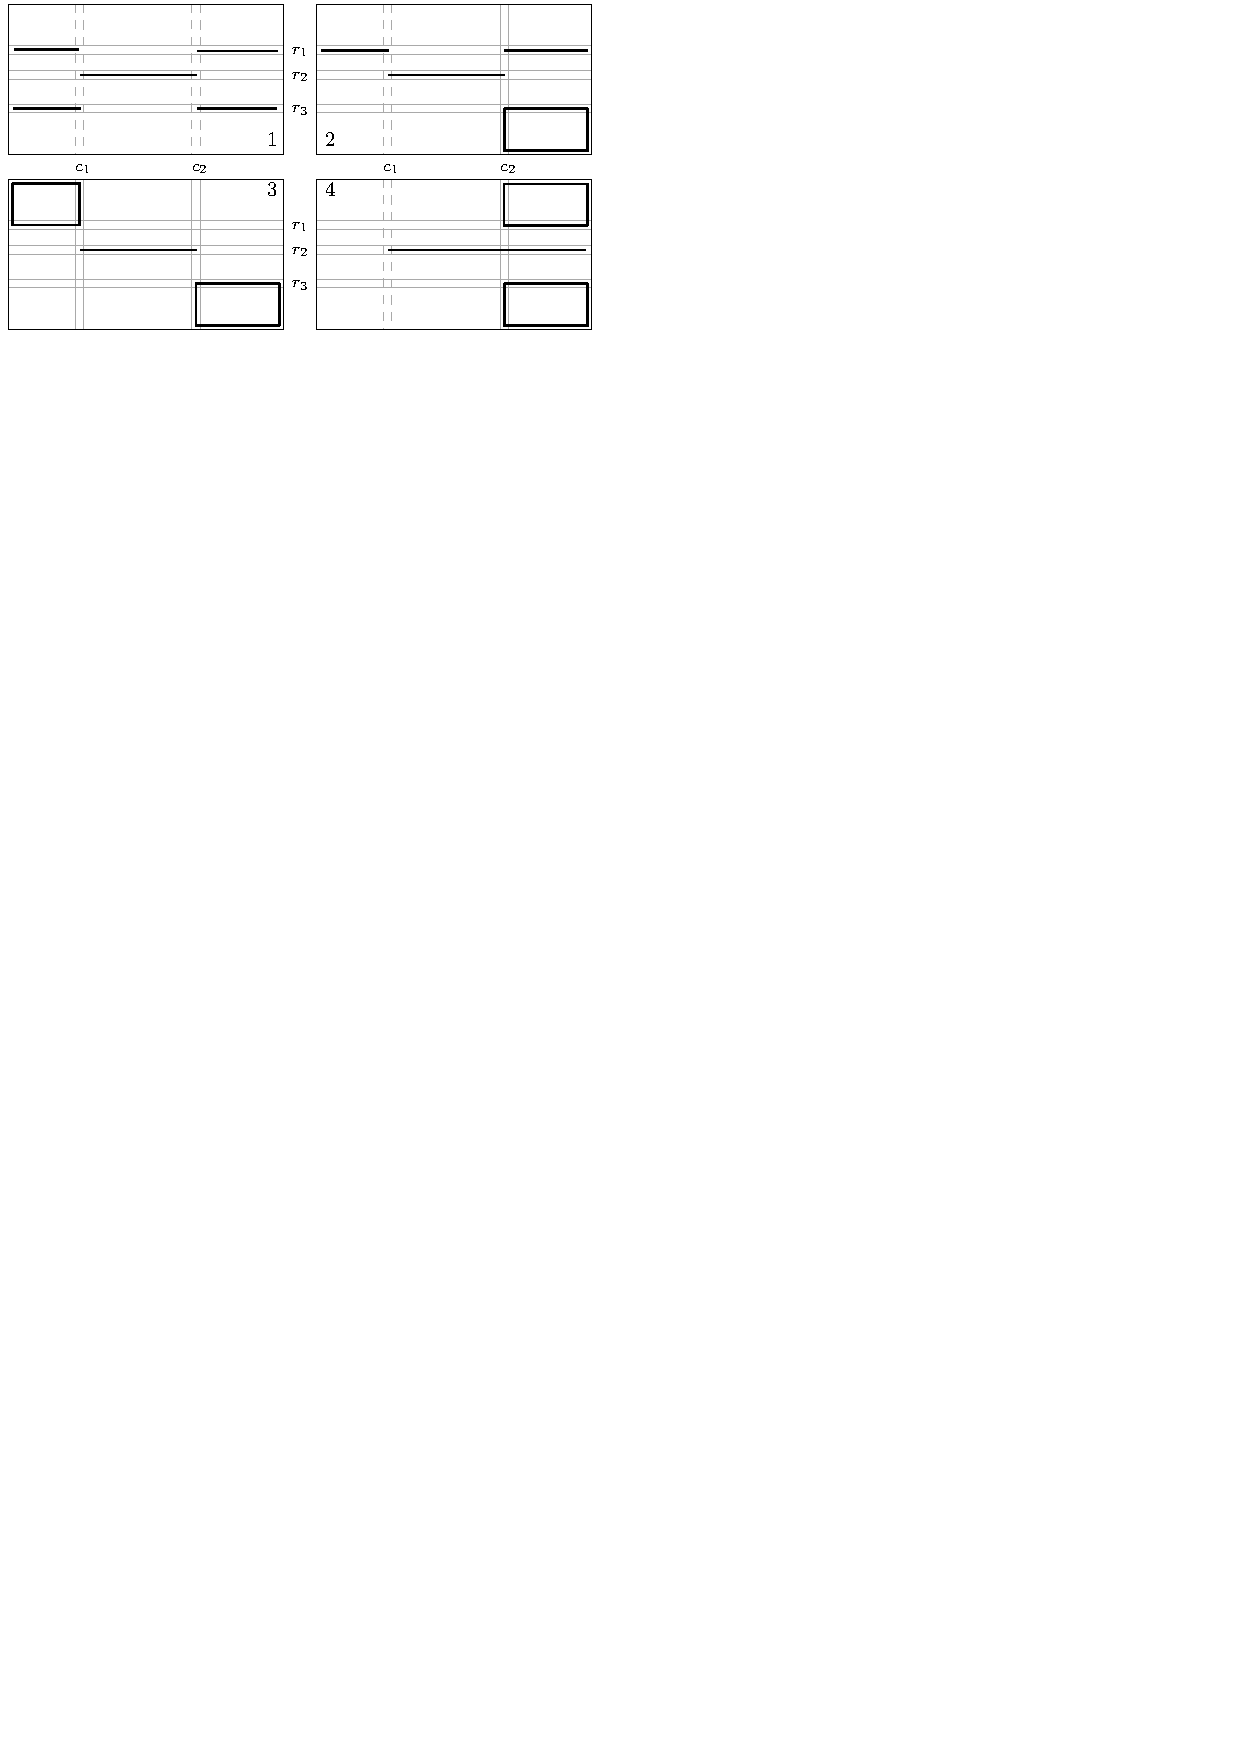
\includegraphics[width=\textwidth]{img/lemmaH.pdf}
\caption{Patterns for which one-entries in row~$r_2$ and columns $c_1$ to $c_2$ are row-bounded. One-entries may only be in the areas enclosed by bold lines.}
\label{fig:lemmaH}
\end{figure}
\end{lemma}
\begin{proof}
Let $P$ be the first described pattern and let $k'=c_2-c_1$. We show that for each one-entry $e$ from row~$r_2$ and every $M\in\Avmax{P}$ there is at most $k'$ zero-intervals for which it is usable. For contradiction assume there is a row~$r$ with $k'+1$ zero-intervals usable for $e$. It follows that there are at least $k'$ one-entries in between two most distant zero-intervals $z_1$ and $z_2$. Therefore, the whole row~$r_2$ can be mapped just to $r$. Since changing a zero-entry of $z_1$ to a one-entry to which $e$ can be mapped creates a partitioning of $M$ where all one-entries from columns $1$ to $c_1$ are mapped to columns up to $z_1$ and similarly all one-entries from columns $c_2$ to $l$ can be mapped to columns from and past $z_2$, we can simply map empty rows from $r_1+1$ to $r_3-1$ around row $r$ and use the rest to map rows $r_1$ and $r_2$. Described partitioning gives us $\PimM$ and a contradiction. We can see the partitioning in Figure~\ref{fig:lemmaH1}.
\begin{figure}[!ht]
\centering
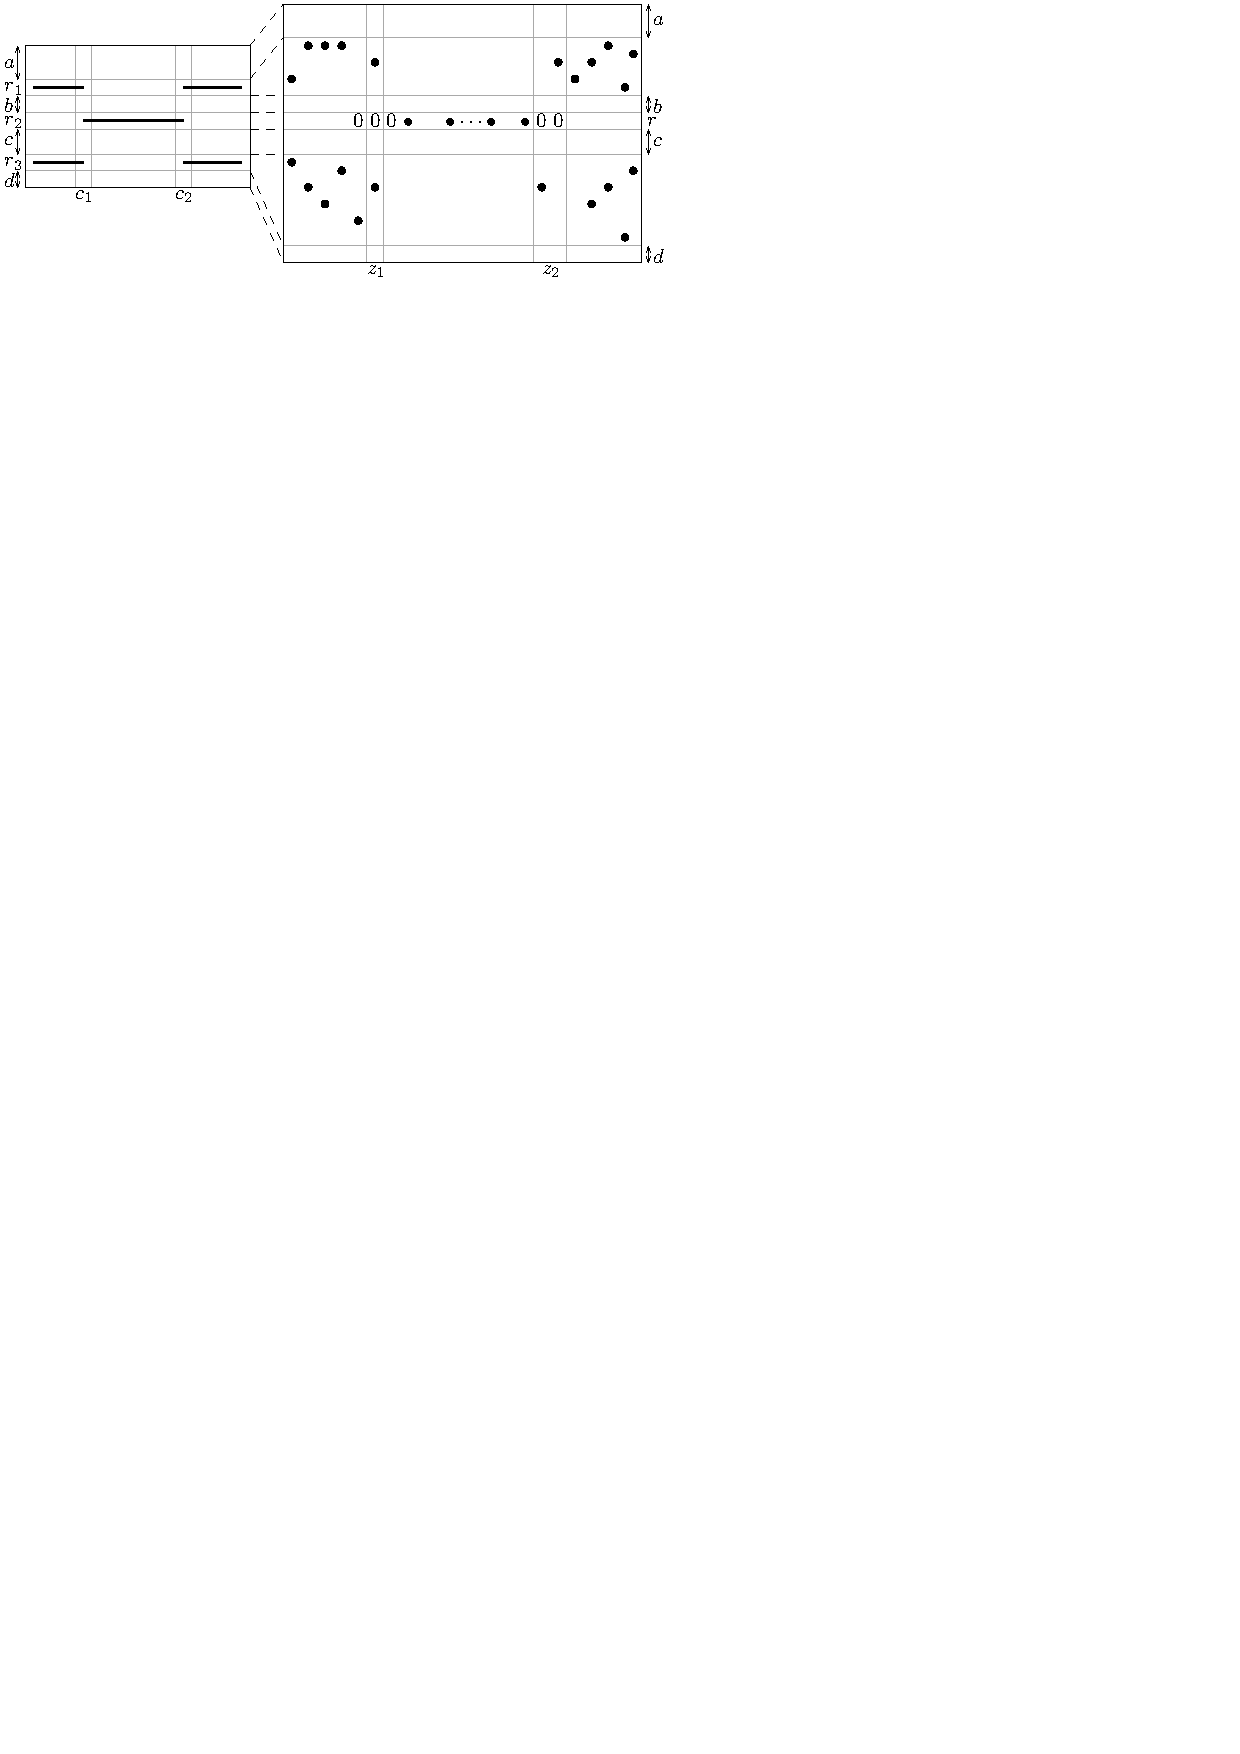
\includegraphics[width=\textwidth]{img/lemmaH1.pdf}
\caption{Mapping of a pattern into a matrix only using one line to map an empty line of the pattern and only using one line to map row~$r_2$.}
\label{fig:lemmaH1}
\end{figure}

Proofs of cases two and three are similar to the first one and we skip them.

Let us look on the fourth case. For $i$-th one-entry in row~$r_2$ (ordered from left to right and only considering those in columns $c_1$ to $c_2$) no zero-interval of a maximal matrix avoiding the pattern cannot have $i$ one-entries to the left of it and so each such one-entry is bounded by $i\geq l$.

It is important to realize we could not have used the same proof we used for the first three cases also for the fourth case, because we can never rely on the fact a mapping of $P$ only uses one row of $M$ to map row~$r_2$. This is because in the fourth case, unlike the first three, there are also potential one-entries in $P[\{r_2\},[c_2,l]]$.
\end{proof}

%%%%%%%%%%%%%%%%%%%%%%%%%%%%%%%%%%%%%%%%%%%% Lemma I
\begin{lemma}
\label{lemma:I}
Let $P\in\Pat$ be a pattern structured like one of the matrices in Figure~\ref{fig:lemmaI}. Then every one-entry in $P[[r_1+1,r_2-1],\{c\}]$ is row-bounded.

\begin{figure}[!ht]
\centering
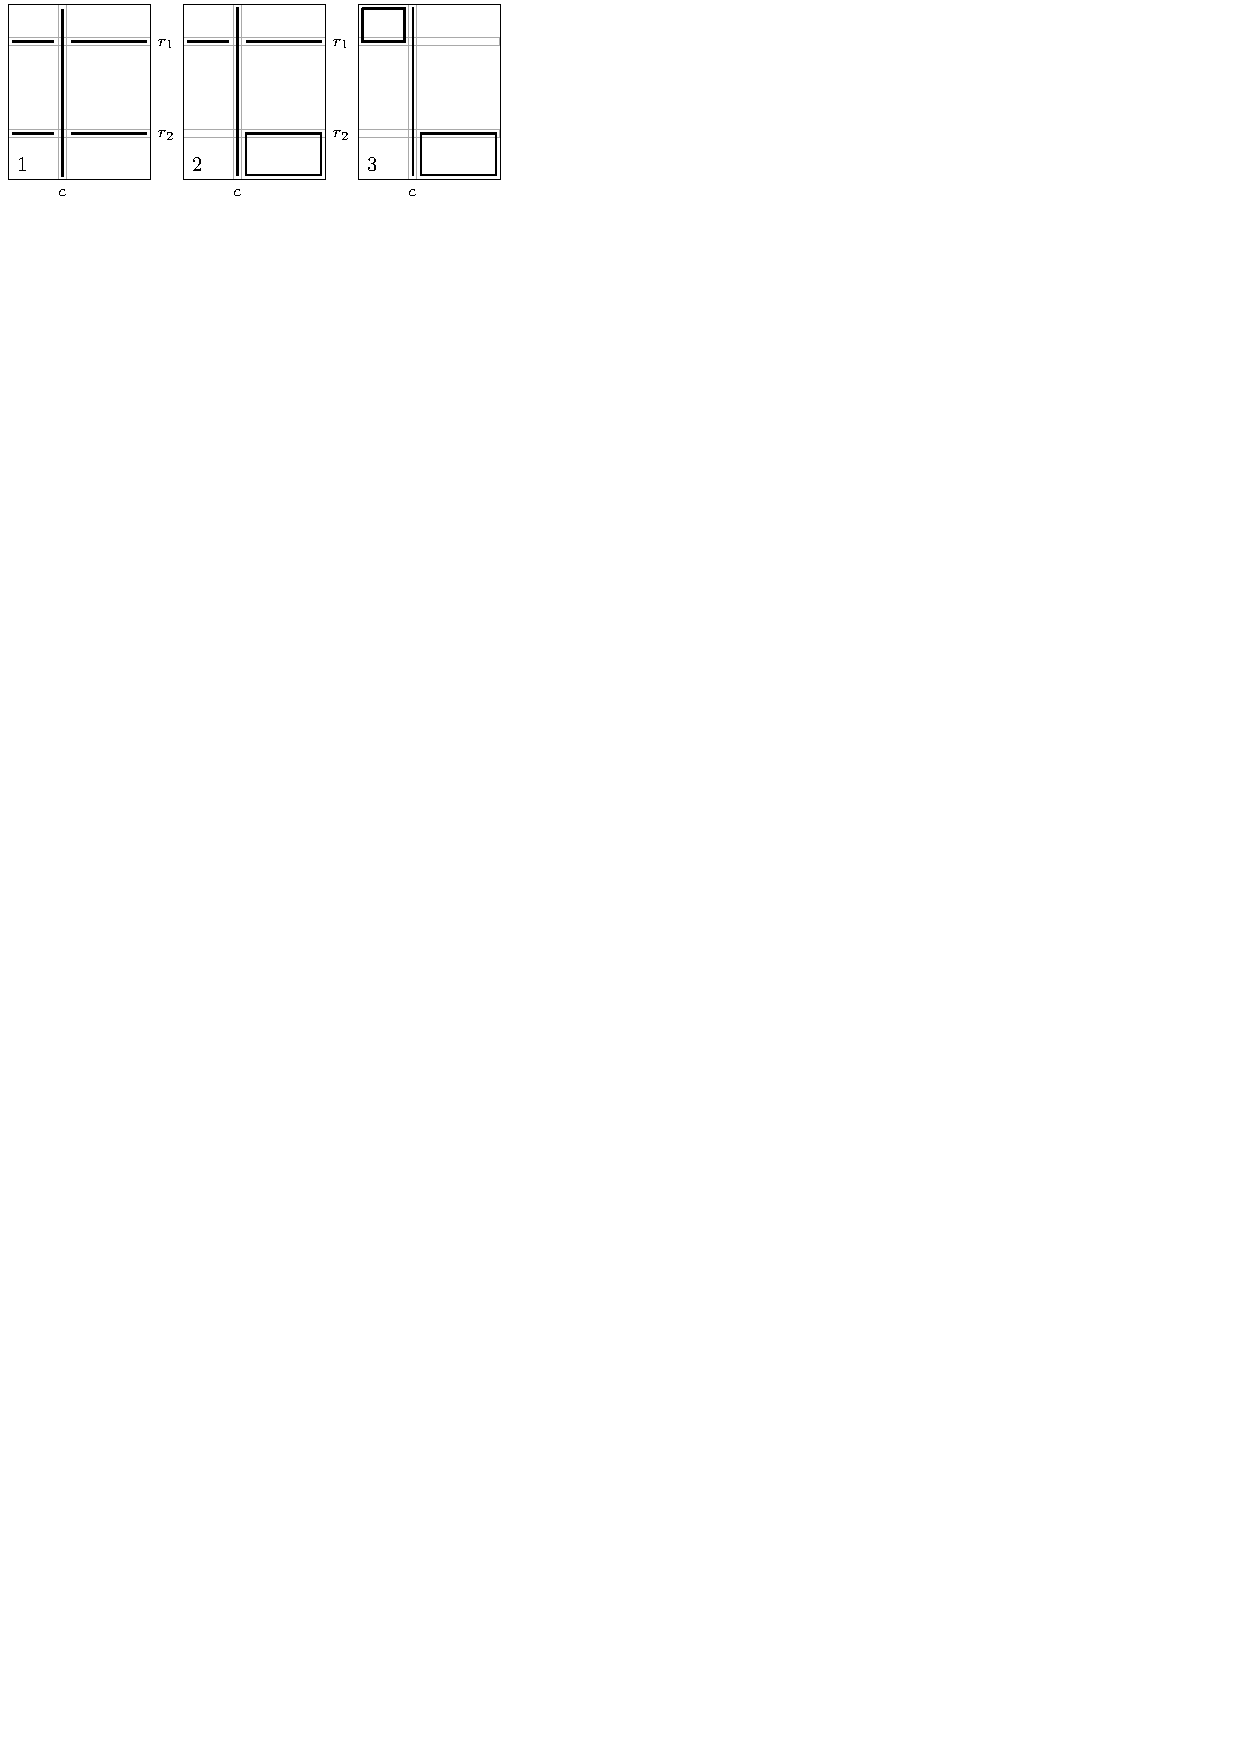
\includegraphics[width=120mm]{img/lemmaI.pdf}
\caption{Patterns for which one-entries in column~$c$ and rows $r_1+1$ to $r_2-1$ are row-bounded. One-entries may only be in the areas enclosed by bold lines.}
\label{fig:lemmaI}
\end{figure}
\end{lemma}
\begin{proof}
Let $P$ be the first described pattern. We show that for each one-entry from $P[[r_1+1,r_2-1],\{c\}]$ and every $M$ maximal matrix avoiding $P$ there is at most one zero-interval for which it is usable. For contradiction assume there is a row~$r$ with two zero-intervals $z_1$ and $z_2$ usable for $e$. Look at Figure~\ref{fig:lemmaI1} and let the dashed partitioning be a mapping of $P$ to $M$ when a zero-entry of $z_1$ is changed to a one-entry used to map $e$ and let the dotted partitioning be a mapping of $P$ to $M$ when a zero-entry of $z_2$ is changed to a one-entry used to map $e$. If we map column $c$ to where it is mapped in both mappings together and map rows $r_1$ and $r_2$ as suggested in the picture, we get a partitioning of $P$ inside $M$ and so a contradiction with $\PnimM$.

\begin{figure}[!ht]
\centering
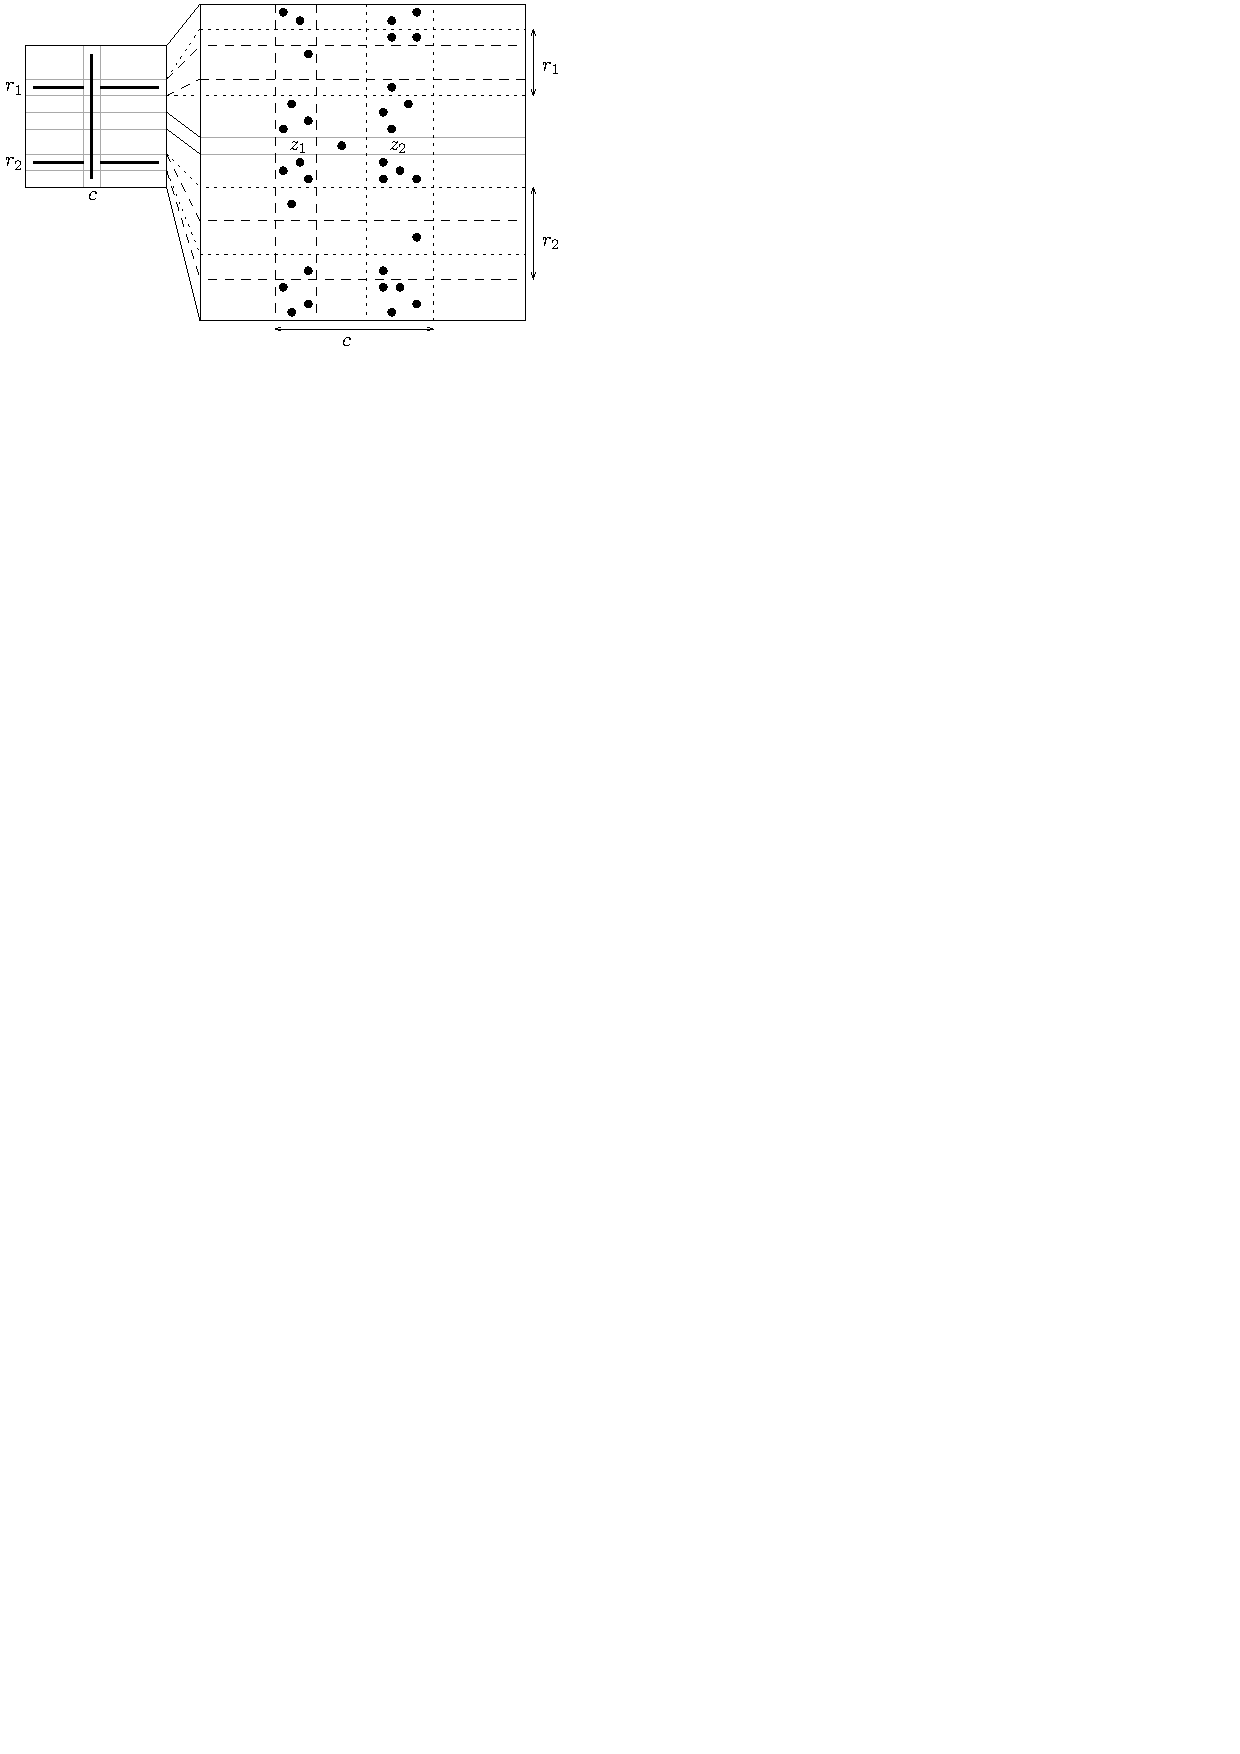
\includegraphics[width=100mm]{img/lemmaI1.pdf}
\caption{}
\label{fig:lemmaI1}
\end{figure}

Proofs of cases two and three are similar to the first one and we skip them.
\end{proof}

%%%%%%%%%%%%%%%%%%%%%%%%%%%%%%%%%%%%%%%%%%%%%% First non-empty column bounded
\begin{lemma}
\label{lemma:First}
Let $P$ be a pattern and $c$ be its first non-empty column. Then every one-entry from $c$ is row-bounded.
\end{lemma}
\begin{proof}
The result follows immediately from the fourth case of Lemma~\ref{lemma:H}.
\end{proof}

%%%%%%%%%%%%%%%%%%%%%%%%%%%%%%%%%%%%%%%%%% walking patterns
\begin{lemma}
\label{lemma:walkpat}
Let $P\in\Pat$ be a pattern avoiding $\smm{ &\bullet\\\bullet& }$ (or $\smm{\bullet& \\ &\bullet}$). Then $\Avm{P}$ is bounded.
\end{lemma}
\begin{proof}
From Proposition~\ref{prop:walking} we know that $P$ is a walking pattern. Every one-entry of $P$ satisfies either conditions of the third case of Lemma~\ref{lemma:H} or it satisfies conditions of the third case of Lemma~\ref{lemma:I} and therefore is row-bounded. From Observation~\ref{obs:transposebounded}, we know it is also column-bounded.
\end{proof}

%%%%%%%%%%%%%%%%%%%%%%%%%%%%%%%%%%%%%%%%%%% three non-empty lines - it is super long
\begin{lemma}
Let $P\in\Pat$ be a pattern having three non-empty lines and avoiding all rotations of $P_1$. Then $\Avm{P}$ is bounded.
\end{lemma}
\begin{proof}
First of all, if $P$ avoids $\smm{ &\bullet\\\bullet& }$ or $\smm{\bullet& \\ &\bullet}$, we use Lemma~\ref{lemma:walkpat}. From now on, we assume it contains both.

Let us prove that each pattern having one-entries in three rows is bounded. Pattern $P$ has one-entries in at least three columns; therefore, it contains a three by three permutation matrix as a submatrix. Since rotations of $P_1$ are avoided, only feasible permutations are 123 and 321 and without loss of generality we assume the first case. In Figure~\ref{fig:threelines} we see the structure of each such pattern. Capital letters stand for one-entries of the permutation, letters $a-f$ stand each for a potential one-entry and Greek letters stand each for a potential sequence of one-entries and zero-entries. Everything else is empty. Not all one-entries can be there at the same time, because that would create a mapping of $P_1$ or its rotation. We also need to find $\smm{\bullet& \\ &\bullet}$. The following analysis only uses hereditary arguments, which means that if we prove $P$ is bounded, we also prove that each submatrix of $P$ is bounded. With this in mind, we restrict ourselves to maximal patterns.
\begin{figure}[!ht]
	\centering
	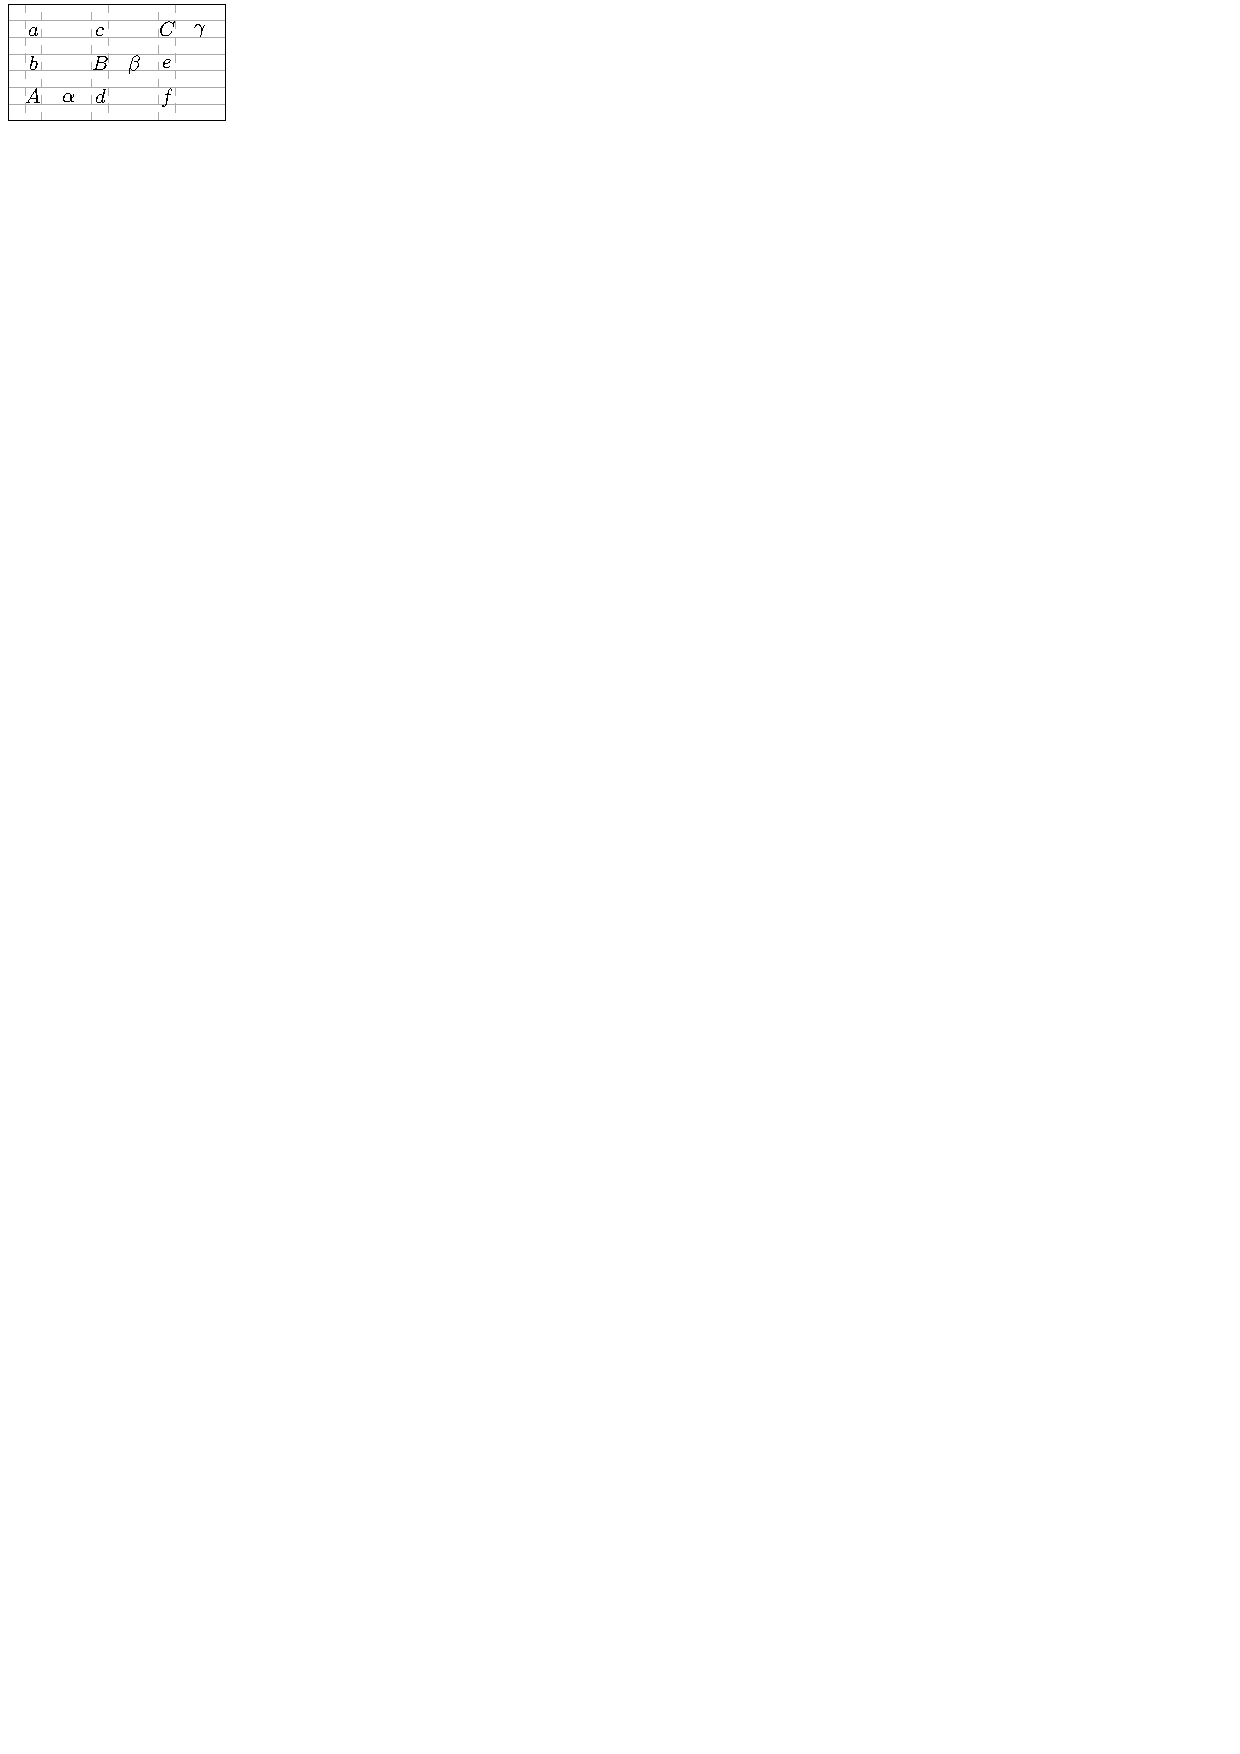
\includegraphics[width=70mm]{img/threelines.pdf}
	\caption{Structure of a pattern only having three non-empty rows and avoiding all rotations of $P_1$.}
	\label{fig:threelines}
\end{figure}

Before we start going through cases, it is easy to see that from the fourth case of Lemma~\ref{lemma:H}, all one-entries in $a,b,A,C$ and $\gamma$ are row-bounded. Similarly, from Lemma~\ref{lemma:First}, we have that one-entries in $a,c,d,A,C$ and $\gamma$ are column-bounded.
\begin{itemize}
	\item $\gamma$ contains a one-entry $\Rightarrow f=0\Rightarrow$ because $\smm{\bullet& \\ &\bullet}$ needs to be there it holds $a=1\Rightarrow\alpha=0$
		\begin{itemize}
			\item $d=1\Rightarrow b=0,\ \beta=0,\ e=0$:\\
				Lemma~\ref{lemma:H} (case 4): $c$ is row-bounded.\\
				Lemma~\ref{lemma:I} (case 1): $B$ is row-bounded.\\				
				\textbf{TODO} what about $d$?\\
				
				Lemma~\ref{lemma:H} (case 1): $B$ is column-bounded.
			\item $d=0$
				\begin{itemize}
					\item $c=1\Rightarrow\beta=0,\ e=0$:\\
						Lemma~\ref{lemma:H} (case 4): $c$ is row-bounded.\\
						Lemma~\ref{lemma:H} (case 1): $B$ is row-bounded.\\
						
						Lemma~\ref{lemma:H} (case 2): $b,B$ are column-bounded.
					\item $c=0$:\\
						Lemma~\ref{lemma:H} (case 1): one-entries in $b,e,B$ and $\beta$ are row-bounded.\\
						
						Lemma~\ref{lemma:I} (case 2): one-entries in $B$ and $\beta$ are column-bounded.\\
						\textbf{TODO} what about $b,e$?
				\end{itemize}
		\end{itemize}
	\item $\gamma=0$: one-entries in $e$ and $f$ are row-bounded from Lemma~\ref{lemma:First}.
		\begin{itemize}
			\item $\alpha$ contains a one-entry $\Rightarrow a=0,\ b=0$:\\
				The pattern is rotation symmetric around $\beta$ and we have already gone through all cases.
			\item $\alpha=0$:\\
				Without loss of generality, we assume that $a=1$, because there needs to be $\smm{\bullet& \\ &\bullet}$ and if we set $a=0$, it must hold $f=1$ and then we can just rotate the pattern by 180 degrees and get the case $a=1$.
				\begin{itemize}
					\item $c=1,\ d=1\Rightarrow b=0,\ e=0,\ \beta=0$
						Lemma~\ref{lemma:I} (case 1): $B$ is row-bounded.\\
						\textbf{TODO} what about $c,d$?\\
						
						Lemma~\ref{lemma:H} (case 1): $B$ is column-bounded.
					\item $c=1,\ d=0\Rightarrow e=0,\ \beta=0$: Without loss of generality, $b=1$. Otherwise, we have the previous case. Therefore, $f=0$.
						Lemma~\ref{lemma:H} (case 4): $c$ is row-bounded.\\
						Lemma~\ref{lemma:H} (case 1): $B$ is row-bounded.\\
						
						Lemma~\ref{lemma:H} (case 4): $b$ is column-bounded.\\
						Lemma~\ref{lemma:H} (case 1): $B$ is column-bounded.
					\item $c=0,\ d=1\Rightarrow b=0$: Without loss of generality, $e=1$ or $\beta$ contains a one-entry. Otherwise, we have the case $c=1,\ d=1$. Therefore, $a=0$.
						Lemma~\ref{lemma:H} (case 4): $d$ is row-bounded.\\
						Lemma~\ref{lemma:H} (case 1): one-entries in $B$ and $\beta$ are row-bounded.\\
						
						Lemma~\ref{lemma:H} (case 1): $B$ is column-bounded.\\
						Lemma~\ref{lemma:I} (case 2): one-entries in $\beta$ are column-bounded.\\
						\textbf{TODO} what about $e$?
					\item $c=0,\ d=0$:
						Lemma~\ref{lemma:H} (case 1): one-entries in $B$ and $\beta$ are row-bounded.\\
						
						Lemma~\ref{lemma:I} (case 1): one-entries in $B$ and $\beta$ are column-bounded.\\
						\textbf{TODO} what about $b,e$?
				\end{itemize}
		\end{itemize}
\end{itemize}
The same analysis also proves that if the pattern with the same restrictions only has three non-empty columns then it is bounded.

Let us now look at the case when all one-entries of the pattern are in either one of two rows $r_1,r_2$ or in a column~$c_1$. Without loss of generality, we again assume permutation 123 is present and we distinguish three cases. Consider Figure~\ref{fig:twoplusone}:
\begin{figure}[!ht]
	\centering
	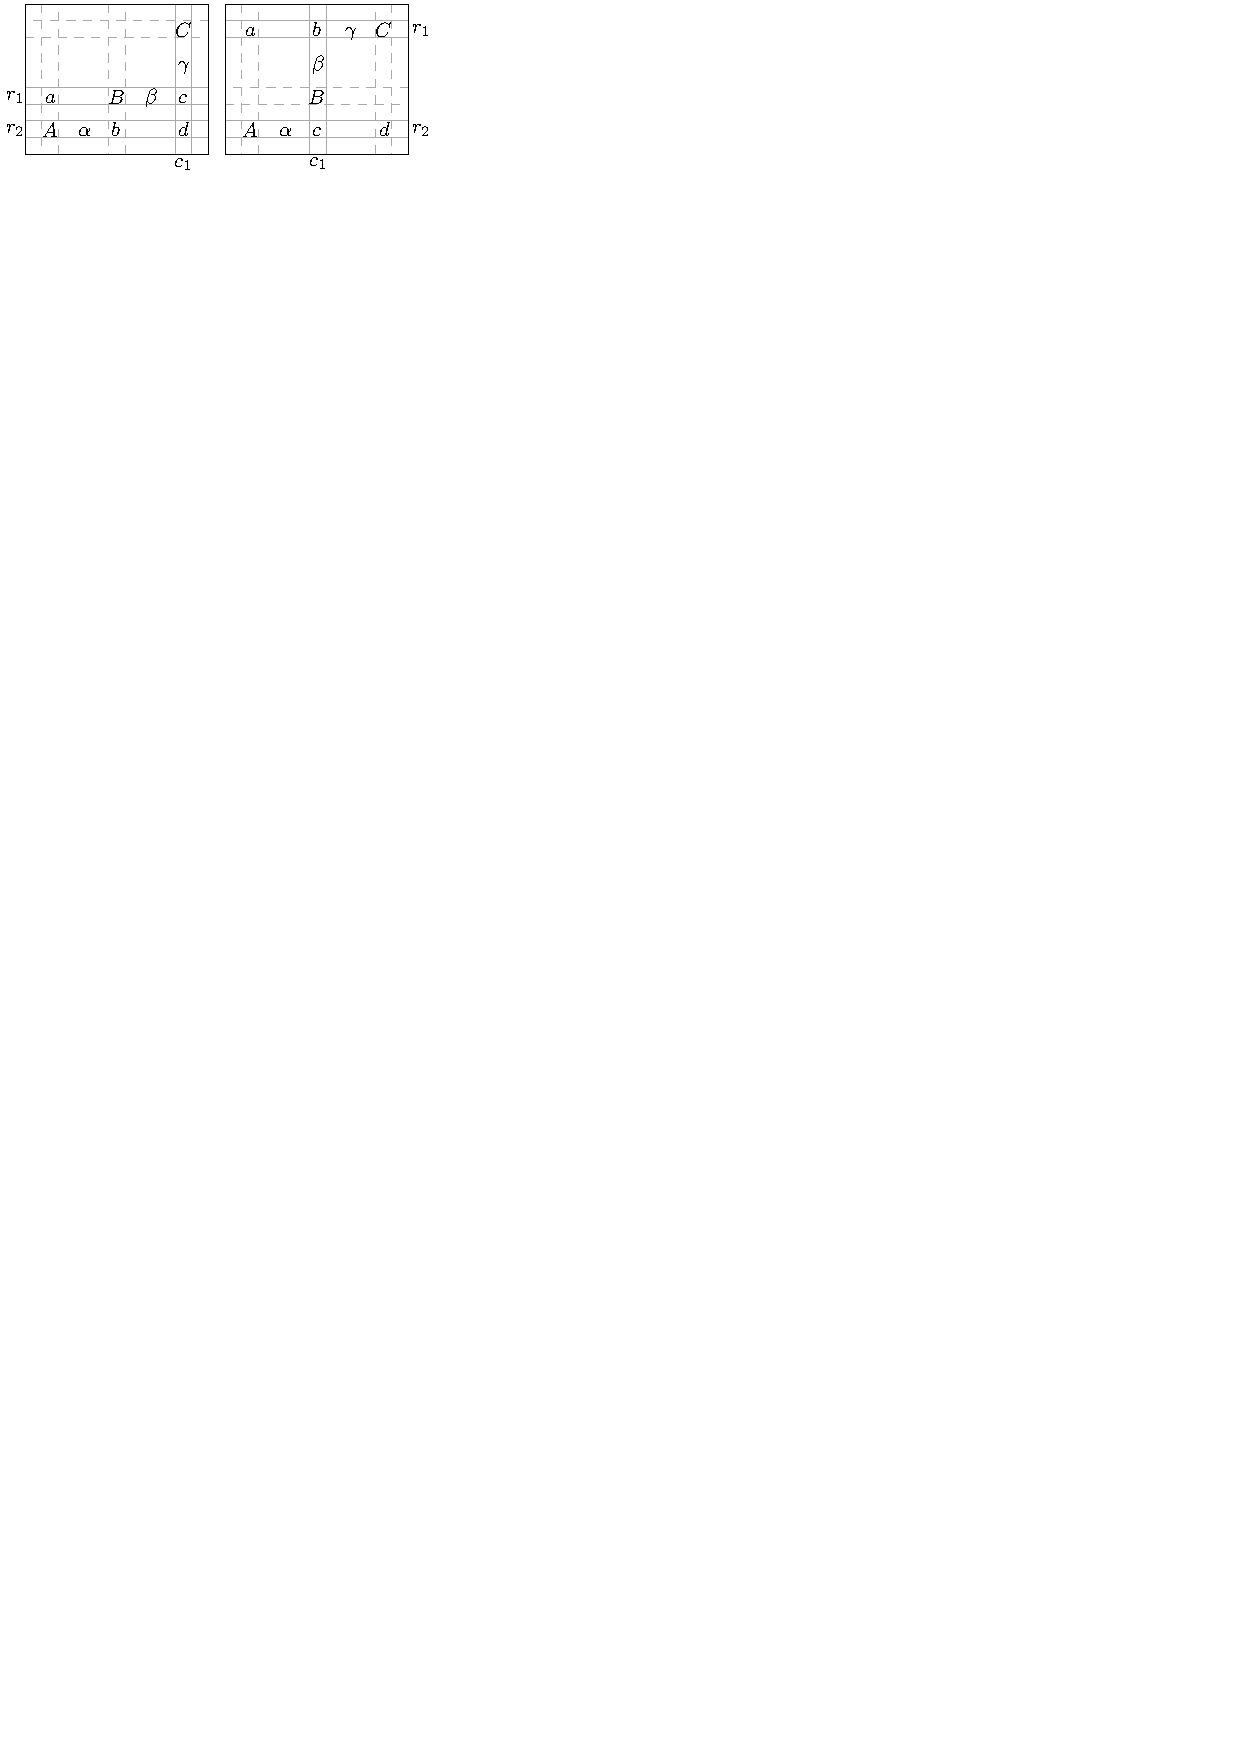
\includegraphics[width=120mm]{img/twoplusone.pdf}
	\caption{Structure of a pattern only having one-entries in two rows and one column that avoids all rotations of $P_1$.}
	\label{fig:twoplusone}
\end{figure}
\begin{itemize}
\item $C$ lies in column~$c_1$: Thanks to Lemma~\ref{lemma:First} are one-entries in $a,c,d,A,C$ and $\gamma$ row-bounded and one-entries in $b,d,A$ and $\alpha$ column-bounded. From the fourth case of Lemma~\ref{lemma:H}, we have that one-entries in $c,C$ and $\gamma$ are column-bounded.
	\begin{itemize}
		\item $a=1\Rightarrow b=0,\ \alpha=0$:\\
			Lemma~\ref{lemma:H} (case 2): one-entries in $B$ and $\beta$ are row-bounded.\\
			
			Lemma~\ref{lemma:I} (case 1): one-entries in $B$ and $\beta$ are column-bounded.\\
			\textbf{TODO} what about $a,c$?
		\item $a=0$:\\
			Lemma~\ref{lemma:H} (case 4): one-entries in $b$ and $\alpha$ are row-bounded.\\
			Lemma~\ref{lemma:H} (case 2): one-entries in $B$ and $\beta$ are row-bounded.\\
			
			Lemma~\ref{lemma:I} (case 2): one-entries in $\beta$ are column-bounded.\\
			\textbf{TODO} what about $c,B$?
	\end{itemize}
\item $B$ lies in column~$c_1$: Thanks to Lemma~\ref{lemma:First} are one-entries in $a,d,A,C$ row-bounded and one-entries in $a,b,c,d,A,C,\alpha$ and $\gamma$ column-bounded. From the first case of Lemma~\ref{lemma:I}, we have that one-entries in $B$ and $\beta$ are row-bounded and from the first case of Lemma~\ref{lemma:H}, one-entries in $b,c,B$ and $\beta$ are column-bounded. Thus, every one-entry is column-bounded.
	\begin{itemize}
		\item $a=1\Rightarrow\alpha=0$
			\begin{itemize}
				\item $d=1\Rightarrow\gamma=0$:\\
					\textbf{TODO} what about $b,c$?\\
				\item $d=0$:\\
					Lemma~\ref{lemma:H} (case 4): one-entries in $b$ and $\gamma$ are row-bounded.\\
					\textbf{TODO} what about $c$?
			\end{itemize}
		\item $a=0$
			\begin{itemize}
				\item $d=1\Rightarrow\gamma=0$:\\
					Lemma~\ref{lemma:H} (case 4): one-entries in $c$ and $\alpha$ are row-bounded.\\
					\textbf{TODO} what about $c$?
				\item $d=0$: The pattern avoids $\smm{\bullet& \\ &\bullet}$ so it is bounded from Lemma~\ref{lemma:walkpat}.
			\end{itemize}
	\end{itemize}
\item $A$ lies in column~$c_1$:\\
	This is symmetric to the first situation.
\end{itemize}
The same analysis also proves that if one-entries of a pattern with the same restrictions are in one row or two columns then the pattern is bounded.
\end{proof}

Combining all the lemmata we finally get the following result.

\begin{thm}
Let $P$ be a pattern avoiding all rotations of $P_1$, then $\Avm{P}$ is bounded. \qed
\end{thm}

\section{Chain rules}
In this section, we study what happens when we combine multiple classes that are bounded or unbounded.

\begin{thm}
\label{thm:boundunion}
Let $\mathcal{P}$ and $\mathcal{Q}$ be classes of patterns. If both $\mathcal{P}$ and $\mathcal{Q}$ are bounded then $Av(\mathcal{P}\cup\mathcal{Q})$ is bounded.
\end{thm}
\begin{proof}
We show $comp_{\mathcal{P}\cup\mathcal{Q}}\leq comp_\mathcal{P}+comp_\mathcal{Q}=C$.

For contradiction, let $M$ be a maximal matrix avoiding $\mathcal{P}\cup\mathcal{Q}$ having at least $C+1$ zero-intervals in a single row (or column). Without loss of generality it means there is more than $comp_\mathcal{P}$ zero-intervals usable for one-entries of the patterns from $\mathcal{P}$. Not let us change some zero-entries of $M$ to one-entries to get $M'\in Av(\mathcal{P})$. Clearly, it still contains more than $comp_\mathcal{P}$ zero-intervals usable for one-entries of the patterns from $\mathcal{P}$, which is a contradiction with the definition of $comp_\mathcal{P}$.

Similarly, the same inequality holds also for the column-complexity of $\mathcal{P}\cup\mathcal{Q}$ and so the union is bounded.
\end{proof}

Using induction, we can show that also a union of a finite number of bounded classes of finite sizes is bounded. Interestingly enough, unbounded classes are not closed the same way.

\begin{thm}
For every $1\leq i<j\leq4]$ is $\{P_i,P_j\}$ bounded.
\end{thm}
\begin{proof}
Due to symmetries it is enough to only consider $i=1$ and $j=[1,2]$.

\begin{itemize}
	\item $\{P_1,P_2\}$ is row-bounded: from Lemma~\ref{lemma:First} we have that one-entries $P_1[2,1],P_1[3,3],P_2[2,3]$ and $P_3[3,1]$ are row-bounded. For $P_1[1,2]$ and $P_2[1,2]$ we prove there are at most two zero-intervals usable for each of them. Otherwise, if there are three zero-intervals $z_1<z_2<z_3$ usable for $P_1[1,2]$ then the one-entries used to map $P_1[2,1]$ and $P_1[3,3]$ in a mapping created when a zero-entry of $z_1$ changes to one-entry used to map $P_1[1,2]$ together with a one-entry in between $z_2$ and $z_3$ give us a mapping of $P_2$ to $M$. Symmetrically, the same goes for $P_2[1,2]$ and $z'_3$.
	\item $\{P_1,P_2\}$ is column-bounded: from Lemma~\ref{lemma:First} combined with Observation~\ref{obs:transposebounded} we have that one-entries $P_1[1,2],P_1[3,3],P_2[1,2]$ and $P_3[3,1]$ are column-bounded. For $P_1[2,1]$ and $P_2[2,3]$ we prove there are at most two zero-intervals usable for each of them. Otherwise, if there are three zero-intervals $z_1<z_2<z_3$ (from top down) usable for $P_[2,1]$ then the one-entries used to map $P_1[1,2]$ and $P_1[3,3]$ in a mapping created when a zero-entry of $z_1$ changes to one-entry used to map $P_1[1,2]$ together with a one-entry in between $z_2$ and $z_3$ give us a mapping of $P_2$ to $M$. Symmetrically, the same goes for $P_2[2,3]$ and $z'_3$.
	\item $\{P_1,P_3\}$ is row-bounded: we can use the same proof as when showing that $\{P_1,P_2\}$ is column-bounded.
	\item $\{P_1,P_3\}$ is column-bounded: we can use the same proof as when showing that $\{P_1,P_2\}$ is row-bounded.
\end{itemize}
\end{proof}

We prove even stronger result by using a well known fact from the theory of ordered sets.

\begin{fct}[Higman's lemma]
\label{fct:Higman}
Let $A$ be a finite alphabet and $A^*$ be a set of finite sequences over $A$. Then $A^*$ is well quasi ordered with respect to the subsequence relation.
\end{fct}

\begin{thm}
$\sigma=Av\left(\smm{ &\bullet& \\\bullet& & \\ & &\bullet},\smm{ &\bullet& \\ & &\bullet\\\bullet& & },\smm{\bullet& & \\ & &\bullet\\ &\bullet& },\smm{ & &\bullet\\\bullet& & \\ &\bullet& }\right)$ is bounded. Moreover, every subclass is bounded.
\end{thm}
\begin{proof}
From Theorem~\ref{thm:boundedints} we know that elements of $\sigma$ fall into finitely many classes. For each we need to prove that it is bounded and also that it does not contain an infinite anti-chain. Knowing that we use Theorem~\ref{thm:boundunion} to obtain the result. Let us consider an $m$ by $n$ matrix $M\in\sigma$:
\begin{itemize}
	\item $M$ only contains up to three non-empty rows (columns):\\
		Clearly, if $M$ is maximal then it contains three rows made of one-entries and everything else is zero, so the number of one-intervals is bounded by three.\\
		
		We use words over alphabet~$A=\{a,b,c,d,e,f,g,h,i,j\}$ to describe each $M$ as follows. Let $r_1<r_2<r_3$ be the non-empty rows (if less then three are non-empty we choose extra values arbitrarily). We define $w_M\in A^*$ as follows. First, we use letter $g$ $r_1$ times, letter $h$ $r_2-r_1$ times, letter $i$ $r_3-r_2$ times and letter $j$ $m-r_3$ times to describe the number of rows of $M$. Then we describe columns from the first one to the last one as follows. For each 0 in $r_1$ we use letter $a$ and for 1, we use $ab$. For each 0 in $r_2$ we use letter $c$ and for 1, we use $cd$. For each 0 in $r_3$ we use letter $e$ and for 1, we use $ef$.
		
		If we have $w_M,w_{M'}\in A^*$ such that $w_M$ is a subsequence of $w_{M'}$ then we want to show that $M$ is an interval minor of $M'$. Let $r_1,r_2,r_3$ and $r_1',r_2',r_3'$ be the non-empty rows of $M$ and $M'$ respectively. Since the number of leading letters $g$ is not bigger in $w_M$, $M$ does not have more empty rows before $r_1$ than $M'$ does before $r_1'$ and similarly it has at most as many empty rows in between $r_1,r_2$ and $r_2,r_3$ and after $r_3$.

		Now consider there is $ab$ in $w_M$ and it corresponds to some $a\dots b$ in $w_{M'}$. We can always assume that in $w_{M'}$ the ``$a$'' is the one exactly before $b$. It can only happen that $abcdeface$ is a subsequence of $\textbf{ab}cea\textbf{cd}eac\textbf{eface}$ if the bold letters are used and since they correspond to one-entries lying in the following columns, this indeed corresponds to an interval minor (but it clearly does not have to mean that $M$ is a submatrix of $M'$).

		From Fact~\ref{fct:Higman} we have that $A^*$ is well ordered which means that matrices having at most three non-empty rows (columns) are well ordered (the construction can be extended to every fixed number of non-empty rows) and so they does not have an infitely long anti-chain.
	\item one-entries of $M$ lie in at most two rows and one column (or vice versa):\\
		The number of one-intervals of any such maximal $M$ is bounded by two.\\
		
		We use words over alphabet~$A=\{a,b,c,d,e,f,g\}$ and for non-empty rows~$r_1,r_2$ and column~$c_1$ we define $w_M$ as follows. We first encode each column in such a way that for each 0 in $r_1$ we use letter $a$ and for 1, we use $ab$. For each 0 in $r_2$ we use letter $c$ and for 1, we use $cd$. Right before and after the description of column $c_1$ we put letter $g$. Next we encode each row in such a way that for each 0 in $c_1$ we use letter $e$ and for each 1 letters $ef$. Right before and after the descriptions of rows $r_1$ and $r_2$ we again place letter $g$.
		
		Because of the distinct letters for encoding rows and columns we can apply the same analysis as we did in the previous case and since entries at $M[r_1,c_1]$ and $M[r_2,c_1]$ are separated from the rest by a special letter~$g$ there is no way to find a one-entry if it is not there.
	\item $M$ avoids $\smm{ &\bullet\\\bullet& }$ (or $\smm{\bullet& \\ &\bullet}$):\\
		From Proposition~\ref{prop:walking} we know $M$ is a walking matrix and any such maximal matrix only contains at most one one-intervals in each row and column.\\
		
		We use words over alphabet~$A=\{a,b,c,d\}$ and encode $M$ as follows. We choose an arbitrary walk of $M$ containing all one-entries and index its entries as $w_1\dots w_{m+n-1}$. Starting from $w_1$ we encode $w_i$ so that $a$ stands for 0 and $ab$ for 1 if $w_{i+1}$ lies in the same row as $w_i$ and we use $c$ for 0 and $cd$ for 1 if $w_{i+1}$ lies in the same column as $w_i$.
\end{itemize}

In the construction of words corresponding to matrices, we only made sure that $w_M\subseteq w_{M'}\Rightarrow M\im M'$ and the other impication does not hold. A different construction may lead to equivalence, but that is not necessary for our result.

We now use distinct alphabets to discribe different classes and when we given a potentialy infinite class of matrices from $\sigma$, we know that inside each class there is at most finite number of minimal matrices such that all of the rest contain a smaller one inside. Using induction on Theorem~\ref{thm:boundunion}, we have that each class is bounded and by applying induction with Theorem~\ref{thm:boundunion} once again we get that the union of the classes is also bounded.
\end{proof}

\begin{obs}
There exists a bounding pattern~$P$ having an unbounded subset of $Av(P)$.
\end{obs}
\begin{proof}
Let $P=I_n$ (identity matrix) for $n>3$. From Lemma~\ref{lemma:walkpat} we have that $P$ is bounding. On the other hand, $Av(I_n,P_1)$ is unbounded, because the construction used in the proof of Lemma~\ref{lemma:manyints} also works for this class.
\end{proof}

We define matrices to be bounded if they are both row-bounded and column-bounded. From what we proved so far, we see that a pattern $P$ is row-bounded if and only of it is column-bounded. But once we look at collections of patterns, this does not have to be true.

\begin{lemma}
There exists a class of patters~$\mathcal{P}$, which is row-bounded but column-unbounded.
\end{lemma}
\begin{proof}
Let $\mathcal{P}=\left\lbrace P=\smm{ &\bullet& \\\bullet& & \\ &\bullet& \\ & &\bullet},I_4=\smm{\bullet& & & \\ &\bullet& & \\ & &\bullet& \\ & & &\bullet}\right\rbrace$. We can use the same construction as we did in Lemma~\ref{lemma:manyints}, just transposed, to prove $Av(\mathcal{P})$ is column-unbounded.

To prove that $\mathcal{P}$ is row-bounded, we take any $M$ maximal avoiding $\mathcal{P}$ and look at an arbitrary row. In Lemma~\ref{lemma:walkpat} we proved that patterns avoiding $\smm{ &\bullet\\\bullet& }$ are bounded and so every one-entry of $I_4$ is row-bounded. We need to proof the same for $P$. Using Lemma~\ref{lemma:First}, $P[2,1]$ and $P[4,3]$ are row-bounded. Using the first case of Lemma~\ref{lemma:I}, $P[3,2]$ is row-bounded. We prove that there are at most two zero-intervals usable for $P[1,2]$. For contradiction, let there be three -- $z_1<z_2<z_3$. It means there are at least two one-entries $e_1<e_2$ in between them. Now consider the partitioning of $P$ into $M$ when a zero-entry of $z_3$ is changed to one-entry used to map $P[1,2]$. Clearly, the one-entry used for mapping $P[2,1]$ lies under the left one-entry~$e$ bounding $z_3$ or in a latter column; otherwise we could use $e$ to map $P[1,2]$ and find the pattern in $M$. It may happen $e=e_2$, but still $e_1$ and the one-entries used for mapping $P[2,1],P[3,2]$ and $P[4,3]$ together give us a mapping of $I_4$ and so a contradiction with $M\in Av(\mathcal{P})$. It means that each one-entry of $P$ is also row-bounded and $Av(\mathcal{P})$ is row-bounded.
\end{proof}

\section{Complexity of one-entries}
So far we have been working with the whole patterns and determining their complexity. To make the results even more general, we can analyze the complexity of each one-entry.

\begin{lemma}
\label{lemma:cross}
Let $P\in\Pat$ be a pattern such that all its one-entries are either in rows $r_1<r_2$ or in $P[[r_2],\{c\}]$. Then $P[r_1,c]$ is row-bounded.
\end{lemma}
\begin{proof}
We prove there are at most $k^4$ zero-intervals usable for $P[r_1,c]$ in each row of any maximal matrix $M$ avoiding $P$. For contradiction, let there be more than $k^4$ of them ($zi_1,\dots,zi_{k^4}$) in some row and for each of them, consider the top most row $r'_j$ used to map $r_2$-th row of $P$ in a mapping created when a zero-entry of $zi_j$ is changed to a one-entry used to map $P[r_1,c]$. Then pairs $[zi_1,r'_1],[zi_2,r'_2],\dots,[zi_{k^4},r'_{k^4}]$ form a sequence of distinct pairs and thanks to the Pidgeonhole principle, there is a subsequence of length at least $k^2$ such that the values of $r'_j$ are either non-increasing or non-decreasing. Without loss of generality, assume they are non-decreasing and let $zi'_1,\dots,zi'_{k^2}$ be their corresponding zero-intervals.

What if $P[r_2,c]=0$? TODO
\end{proof}

\begin{lemma}
\label{lemma:unbound}
Let $P=\smm{ &\bullet&\bullet& \\\bullet& & &\bullet\\ & &\bullet& }$. For every $n>1$ there is a maximal matrix $M$ avoiding $P$ as an interval minor having $n$ zero-intervals usable for $P[1,3]$.
\end{lemma}
\begin{proof} Let $M$ be a $(2n-1)\times(2n-1)$ matrix described by the picture:
$$\smm{	 & &\circ& &\bullet& & &\circ& &\bullet&\cdots&\bullet& & &\circ& &\bullet&\bullet&\bullet&\circ&\bullet\\
		 & & & & & & & & & &\cdots& & & & & & &\bullet&\bullet&\bullet&\bullet\\
		 & & & & & & & & & &\cdots& &\bullet&\bullet& &\bullet& &\bullet&\bullet&\bullet&\bullet\\
		 & & & & & & & & & &\cdots& &\bullet&\bullet&\bullet&\bullet& & & & & \\
		 & & & & & & & & & &\cdots& &\bullet&\bullet&\bullet&\bullet& & & & & \\
		\vdots&\vdots&\vdots&\vdots&\vdots&\vdots&\vdots&\vdots&\vdots&\vdots&\vdots&\vdots&\vdots&\vdots&\vdots&\vdots&\vdots&\vdots&\vdots&\vdots&\vdots\\
		 & & & & &\bullet&\bullet& &\bullet& &\cdots& & & & & & & \\
		 & & & & &\bullet&\bullet&\bullet&\bullet& &\cdots& & & & & & & \\
		\bullet&\bullet& &\bullet& &\bullet&\bullet&\bullet&\bullet& &\cdots& & & & & & & \\
		\bullet&\bullet&\bullet&\bullet& & & & & & &\cdots& & & & & & & \\
		\bullet&\bullet&\bullet&\bullet& & & & & & &\cdots& & & & & & & \\
		 }$$
We see that $\PnimM$ because we always need to map $P[2,1]$ and $P[3,3]$ to just one ``block'' of one-entries of $M$ which only leaves a zero-entry where we need to map $P[1,3]$ or $P[2,4]$.

When we change any marked zero-entry of the first row into a one-entry we get a matrix containing a minor of $\{1\}^{3\times4}$; therefore, containing $P$ as an interval minor. In case $M$ is not maximal, we can add some more one-entries to make it maximal but it will still contain a row with $n$ one-intervals.
\end{proof}

\begin{lemma}
\label{lemma:unbound2}
Let $P=\smm{\bullet& & & & \\ &\bullet& &\bullet& \\ & &\bullet& & \\ & & & &\bullet}$ and $P'=\smm{\bullet& & & & \\ &\bullet& &\bullet& \\ & & & &\bullet\\ & &\bullet& & }$. For every $n>1$ there is a maximal matrix $M$ avoiding both $P$ and $P'$ as an interval minor having $n$ zero-intervals usable for $P[2,2]$ and $P'[2,2]$. Moreover, for every pattern containing $P$ or $P'$ as a submatrix, the one-entry that can be used to map $P[2,2]$ or $P'[2,2]$ is also row-unbounded.
\end{lemma}
\begin{proof} Let $M$ be a $(2n-1)\times(2n-1)$ matrix described by the picture:
$$\smm{	 & & & & & & & & & & & &\cdots& & & & & & & &\bullet&\bullet&\bullet&\bullet&\bullet\\
		 & & & & & & & & & & & &\cdots& & & & & & & &\bullet& &\bullet&\bullet&\bullet\\
		 & & & & & & & & & & & &\cdots& &\bullet&\bullet&\bullet&\bullet&\bullet& & \\
		 & & & & & & & & & & & &\cdots& &\bullet& &\bullet&\bullet&\bullet& & \\
		\vdots&\vdots&\vdots&\vdots&\vdots&\vdots&\vdots&\vdots&\vdots&\vdots&\vdots&\vdots&\vdots&\vdots&\vdots&\vdots&\vdots&\vdots&\vdots&\vdots&\vdots&\vdots&\vdots&\vdots&\vdots\\
		 & & & & & &\bullet&\bullet&\bullet&\bullet&\bullet& &\cdots& & & & & \\
		 & & & & & &\bullet& &\bullet&\bullet&\bullet& &\cdots& & & & & \\
		\bullet&\bullet&\bullet&\bullet&\bullet& & & & & & & &\cdots& & & & & \\
		\bullet& &\bullet&\bullet&\bullet& & & & & & & &\cdots& & & & & \\
		 &\circ& & & &\bullet& &\circ& & & &\bullet&\cdots&\bullet& &\circ& & & &\bullet& &\circ& & & \\
		 & & & & & & & & & & & &\cdots& & & & & & & &\bullet&\bullet&\bullet&\bullet&\bullet\\
		 & & & & & & & & & & & &\cdots& & & & & & & &\bullet&\bullet&\bullet&\bullet&\bullet\\
		 & & & & & & & & & & & &\cdots& &\bullet&\bullet&\bullet&\bullet&\bullet& & \\
		 & & & & & & & & & & & &\cdots& &\bullet&\bullet&\bullet&\bullet&\bullet& & \\
		\vdots&\vdots&\vdots&\vdots&\vdots&\vdots&\vdots&\vdots&\vdots&\vdots&\vdots&\vdots&\vdots&\vdots&\vdots&\vdots&\vdots&\vdots&\vdots&\vdots&\vdots&\vdots&\vdots&\vdots&\vdots\\
		 & & & & & &\bullet&\bullet&\bullet&\bullet&\bullet& &\cdots& & & & & \\
		 & & & & & &\bullet&\bullet&\bullet&\bullet&\bullet& &\cdots& & & & & \\
		\bullet&\bullet&\bullet&\bullet&\bullet& & & & & & & &\cdots& & & & & \\
		\bullet&\bullet&\bullet&\bullet&\bullet& & & & & & & &\cdots& & & & & \\
		 }$$
We see that $\PnimM$.

When we change any marked zero-entry of the middle row into a one-entry we get a matrix containing $\{1\}^{4\times5}$; therefore, both containing $P$ and $P'$ as an interval minor. In case $M$ is not maximal, we can add some more one-entries to make it maximal but it will still contain a row with $n$ one-intervals.

TODO general argument for bigger patterns.
\end{proof}

\begin{lemma}
\label{lemma:unbound3}
Let $P=\smm{\bullet& & & \\ &\bullet&\bullet& \\ &\bullet& & \\ & & &\bullet}$ and $P'=\smm{\bullet& & & \\ &\bullet&\bullet& \\ & & &\bullet\\ &\bullet& & }$. For every $n>1$ there is a maximal matrix $M$ avoiding both $P$ and $P'$ as an interval minor having $n$ zero-intervals usable for $P[2,2]$ and $P'[2,2]$.
\end{lemma}
\begin{proof} Let $M$ be a $(2n-1)\times(2n-1)$ matrix described by the picture:
$$\smm{	 & & & & & & & & & &\cdots& & & & & & &\bullet&\bullet&\bullet&\bullet\\
		 & & & & & & & & & &\cdots& & & & & & &\bullet& &\bullet&\bullet\\
		 & & & & & & & & & &\cdots& &\bullet&\bullet&\bullet&\bullet& & \\
		 & & & & & & & & & &\cdots& &\bullet& &\bullet&\bullet& & \\
		\vdots&\vdots&\vdots&\vdots&\vdots&\vdots&\vdots&\vdots&\vdots&\vdots&\vdots&\vdots&\vdots&\vdots&\vdots&\vdots&\vdots&\vdots&\vdots&\vdots&\vdots\\
		 & & & & &\bullet&\bullet&\bullet&\bullet& &\cdots& & & & & \\
		 & & & & &\bullet& &\bullet&\bullet& &\cdots& & & & & \\
		\bullet&\bullet&\bullet&\bullet& & & & & & &\cdots& & & & & \\
		\bullet& &\bullet&\bullet& & & & & & &\cdots& & & & & \\
		 &\circ& & &\bullet& &\circ& & &\bullet&\cdots&\bullet& &\circ& & &\bullet& &\circ& & \\
		 & & & & & & & & & &\cdots& & & & & & &\bullet&\bullet&\bullet&\bullet\\
		 & & & & & & & & & &\cdots& & & & & & &\bullet&\bullet&\bullet&\bullet\\
		 & & & & & & & & & &\cdots& &\bullet&\bullet&\bullet&\bullet& & \\
		 & & & & & & & & & &\cdots& &\bullet&\bullet&\bullet&\bullet& & \\
		\vdots&\vdots&\vdots&\vdots&\vdots&\vdots&\vdots&\vdots&\vdots&\vdots&\vdots&\vdots&\vdots&\vdots&\vdots&\vdots&\vdots&\vdots&\vdots&\vdots&\vdots\\
		 & & & & &\bullet&\bullet&\bullet&\bullet& &\cdots& & & & & \\
		 & & & & &\bullet&\bullet&\bullet&\bullet& &\cdots& & & & & \\
		\bullet&\bullet&\bullet&\bullet& & & & & & &\cdots& & & & & \\
		\bullet&\bullet&\bullet&\bullet& & & & & & &\cdots& & & & & \\
		 }$$
We see that $\PnimM$.

When we change any marked zero-entry of the middle row into a one-entry we get a matrix containing $\{1\}^{4\times5}$; therefore, containing $P$ as an interval minor. In case $M$ is not maximal, we can add some more one-entries to make it maximal but it will still contain a row with $n$ one-intervals.
\end{proof}

\begin{thm}
Let $P$ be a pattern. Any one-entry $P[r,c]$ is row-unbounded if (and only if) there is a trivially unbounded one-entry $P[r,c']$ and we cannot apply the fourth case of Lemma~\ref{lemma:H} nor Lemma~\ref{lemma:cross} to $P[r,c]$.
\end{thm}
\begin{proof}
Without loss of generality, let $P[r,c']$ be part of mapping of $P_1$, where $P_1[1,2]$ is mapped to it. Let $P_1[2,1]$ be mapped to $P[r_2,c_2]$ and $P_1[3,3]$ be mapped to $P[r_3,c_3]$. We go through all potential one-entries $P[r,c]$ and show that either we can use one of the lemmata mentioned in the statement or the one-entry is row-unbounded.
\begin{itemize}
	\item $c<c_2$: If there is no one-entry in $P[[r-1],[c-1]]$ nor $P[[r+1,k],[c-1]]$, then the fourth case of Lemma~\ref{lemma:H} can be used for $P[r,c]$. Otherwise, first consider there is a one-entry in $P[[r-1],[c-1]]$, then we can use the construction from Lemma~\ref{lemma:unbound2}. In the last case, assume there is a one-entry $P[r',c']$ in $P[[r+1,k],[c-1]]$, then if $r'!=r_2$, entries $P[r,c],P[r',c']$ and $P[r_2,c_2]$ form either $P_1$ or $P_2$ and $P[r,c]$ is trivially row-unbounded. If $r'=r_2$, then we use $P[r,c],P[r',c']$ and $P[r_3,c_3]$ to again find either $P_1$ or $P_2$ and $P[r,c]$ is trivially row-unbounded once again.
	\item $c=c_2$: If there is no one-entry in $P[[r-1],[c-1]]$ nor $P[[r+1,k],[c-1]]$, then the fourth case of Lemma~\ref{lemma:H} can be used for $P[r,c]$. Otherwise, first assume there is a one-entry in $P[[r-1],[c-1]]$, then we can use the construction from Lemma~\ref{lemma:unbound3}. In the last case, assume there is a one-entry $P[r',c']$ in $P[[r+1,k],[c-1]]$, then if $r'!=r_3$, entries $P[r,c],P[r',c']$ and $P[r_3,c_3]$ form either $P_1$ or $P_2$ and $P[r,c]$ is trivially row-unbounded. If $r'=r_3$, then what?
	
	Cannot just use lemma even if it was proved.
	
	TOOD
	\item $c_2<c<c_3$: In this case $P[r,c]$ is trivially unbounded as together with $P[r_2,c_2]$ and $P[r_3,c_3]$ it forms $P_1$.
	\item $c=c_3$: If there is no one-entry in $P[[r-1],[c+1,l]]$ nor $P[[r+1,k],[c+1,l]]$, then the fourth case of Lemma~\ref{lemma:H} can be used for $P[r,c]$. Otherwise, first consider there is a one-entry in $P[[r-1],[c+1,l]]$, then we can use the construction from Lemma~\ref{lemma:unbound3}. In the last case, assume there is a one-entry $P[r',c']$ in $P[[r+1,k],[c-1]]$, then if $r'!=r_2$, entries $P[r,c],P[r',c']$ and $P[r_2,c_2]$ form either $P_1$ or $P_2$ and $P[r,c]$ is trivially row-unbounded. If $r'=r_2$, then we use the construction from Lemma~\ref{lemma:unbound} to show $P[r,c]$ is row-unbounded once again.
	\item $c>c_3$: There are three cases to go through and we can handle them the same way as we did in case $c<c_2$.
\end{itemize}
\end{proof}

Open questions:
\begin{itemize}
	\item Is $\Avm{\smm{ &\bullet& \\\bullet& & \\ & &\bullet},\smm{ &\bullet& \\ & &\bullet\\\bullet& & }}$ \emph{hereditarily} bounded?
	\item Can an non-bounding pattern become bounding after a change of a one-entry to a zero-entry?
\end{itemize}